\documentclass[12pt]{article}
\usepackage{graphicx}
\usepackage{graphics}
\usepackage[percent]{overpic}
\usepackage{hyperref}
\usepackage{indentfirst}
%\usepackage{setspace}
\renewcommand\theequation{{\color{red}\arabic{equation}}}
\hypersetup{colorlinks=true}
\usepackage{amsmath}
\usepackage{empheq}
\usepackage{amsfonts}
\usepackage{float}
\usepackage{algorithm}
\usepackage{algorithmic}
\usepackage{caption}
\usepackage{subfigure}
%\usepackage{subcaption}
\usepackage[numbers]{natbib}
\usepackage{lipsum}
\bibliographystyle{abbrvnat}%{ieeetr}%Choose a bibliograhpic style
\usepackage[toc,page]{appendix}
\addtolength{\textwidth}{1.1in}
\addtolength{\hoffset}{-0.5in}
\addtolength{\textheight}{1.1in}
\addtolength{\voffset}{-0.8in}
\usepackage{tikz,pgfplots}
\usetikzlibrary{arrows,snakes,backgrounds,spy,mindmap,trees}
\usetikzlibrary{er}
%\usepackage{onimage}
\pgfplotsset{compat=newest}
%\usepackage{setspace}
%\doublespacing
%\usepackage{parskip}
%\parskip=2\baselineskip \advance\parskip by 0pt plus 2pt 
\usepackage{rotating}
\newcommand{\mgnote}[1]{\textcolor{magenta}{MG: #1}}
\newcommand{\gsnote}[1]{\textcolor{blue}{GS: #1}}
\newcommand{\vrnote}[1]{\textcolor{red}{VR: #1}}
\newcommand{\IIinv}{{\dot\varepsilon}_{\mathrm{\!\!\:II}}}

\newcommand{\mm}{{\ensuremath{\boldsymbol{m}}}}
\newcommand{\uu}{{\ensuremath{\boldsymbol{u}}}}
\newcommand{\vv}{{\ensuremath{\boldsymbol{v}}}}
\newcommand{\ww}{{\ensuremath{\boldsymbol{w}}}}
\newcommand{\uobs}{{\ensuremath{\boldsymbol{u}_\text{obs}}}}
\newcommand{\ff}{{\ensuremath{\boldsymbol{f}}}}
\newcommand{\FF}{{\ensuremath{\boldsymbol{F}}}}
\newcommand{\ppi}{{\ensuremath{\boldsymbol{\pi}}}}

\newcommand{\ssigma}{{\ensuremath{\boldsymbol{\sigma}}}}
\newcommand{\strain}{{\ensuremath{\dot{\boldsymbol{\varepsilon}}}}}


%\let\oldabstract\abstract
%\let\oldendabstract\endabstract
%\makeatletter
%\renewenvironment{abstract}
%{\renewenvironment{quotation}%
%               {\list{}{\addtolength{\leftmargin}{1em} % change this value to add or remove length to the the default
%                        \listparindent 1.5em%
%                        \itemindent    \listparindent%
%                        \rightmargin   \leftmargin%
%                        \parsep        \z@ \@plus\p@}%
%                \item\relax}%
%               {\endlist}%
%\oldabstract}
%{\oldendabstract}
%\makeatother




\date{}

\title{Chapter 4: Simultaneous inference of plate boundary properties and mantle viscosity with an adjoint optimization with large scale two-dimensional models}


\begin{document}
\maketitle
\begin{abstract}
 Plate motions are a primary surface constraint on forward models of plate and mantle dynamics, rheology, plate boundary stresses, and models for the occurrence of great earthquakes. While plate motions can constrain rheology to a first order, there are also regional constraints on the effective viscosity (from post-glacial rebound and post seismic relaxation). 
We incorporate plate motion and effective viscosity data into an optimization and derive an adjoint, gradients for the inferred parameters, and posterior distributions for the normal and shear stresses within plate boundaries using a Gaussian approximation. 
We apply these methods to 2-D cross-sections of subduction zones, with realistic temperature distributions and fault zone geometries from seismic data. From these models, we analyze the conditional and marginal distributions and find that the 
Tonga and the Marianas sibduction zones have the lowest values of mechanical coupling while Chile and Sumatra the highest, among those studied. The subduction zones with the lowest coupling have back-arc extension. Globally, we find that the non-linear stress-strain exponent, $n$, is 3.0 $\pm$ 0.25 (in the upper mantle and lithosphere) with a pressure-independent yield stress of 150 $\pm$ 25 MPa. The stress in shear zones is tens of MPa and both the shear and the normal stresses are elevated in seismically coupled compared to uncoupled subduction zones and the variations in the inferred mechanical couplings is similar to the variations in observed seismic coupling from previous studies.
\end{abstract} 


\section{Introduction}
While slab pull may be the dominant force driving plate motions and associated mantle flow, there remains substantial uncertainty on the relative coupling of stresses across plate boundaries at subduction zones. This coupling can either be attributed to broad-scale tectonic forces or the varying properties between plates at each subduction zone. While it is not clear whether broad-scale forces or the varying properties have the stronger contribution to the variations in seismic coupling, a valid model should appropriately represent the broad-scale forces. 
Seismic coupling is defined as the ratio between the observed seismic moment release to the rate of plate tectonic velocities and generally varies between 0 and 1 \citep{davies1971regional}. 
Seismic coupling is sensitive to the short window of recorded earthquakes such that if many large magnitude earthquakes occur within that short window 
at a greater rate than the long-term average, then the seismic coupling could be close to or even exceed unity, whereas if the earthquakes occur at an unusally low rate, then the seismic coupling will be small.  While seismic coupling is a reasonable way to build a relationship to forecast which subduction zones have a propensity for future large magnitude events, additional data, for example, the curvature of subduction zones \citep{bletery2016mega} or along strike gravity anomalies \citep{song2003large}, 
can potentially be used to better condition such forecasts. 

  %It was suggested in \citep{ide2013proportionality} that background seismicity can be correlated with subduction zones that have experienced great earthquakes. %Additionally, there might be a correlation between the plate age and b-value \citep{nishikawa2014earthquake}. These results lead to relating the shear and normal stresses (broad-scale forces) at plate boundaries to background seismicity and b-values in addition to the geodetic seismic coupling.

Regardless of whether broad-scale forces or varying shear zone properties are the ultimate cause for variations in seismic coupling, geodynamic models should be able to explain variations between the two end-members from the least coupled Marianas to coupled Chilean subduction zone. The Chilean subduction zone is among the most seismically active with many earthquakes above 8, including the largest ever recorded, the 1960 Valdivia earthquake with magnitude 9.5 magnitude \citep{kanamori1974},
the largest ever recorded. On the other hand the Marianas subduction is among the least seismically coupled with no historic earthquake greater than \mgnote{ need value}. 
Chile, overall is in a state of compression on the South American margin, while, the Marianas subduction zone is characterized by active back arc opening within the Marianas trench indicative of regional tension.


A simple force balance of subduction zones that parameterizes the broad-scale forces suggests a link between tectonic forces and how seismically coupled subduction zones are \citep{scholz1995mechanism, scholz2012seismic}. These models estimate the force distribution that arises from slab pull and a putative anchoring, for each subduction zone. Furthermore, those models do not include key variations in rheology and how such mechanics would influence the distribution of  normal forces.  While the analysis found a relationship between broad-scale forces and coupling, their approach may not capture the essence of the system as the actual geometry of slabs is complex with substantial flow is induced by global flow \citep{scholz2012seismic}. 
Although simple, these force balance models haven't found general acceptance.

%The partitioning of the resisting forces can be seen through the plate-coupling of the weakzone factors in the rheological relationship, which provides the effective frictional resistance in models. There have been investigations into these ideas and how different subduction zones have different fricitional forces.  The notion of coupling can be either mechanical or tectonic coupling. Both ideas can lead to the end member cases 

  To accurately estimate the forces at plate boundaries, not only is the correct physics needed, but an optimization scheme must be constrained by observed plate motion \citep{BursteddeStadlerAlisicEtAl13,Stadler27082010}, the most robust constraint on mantle flow. We overcome these limitations by employing a method similar to our earlier work \citep{ratnaswamy2015adjoint} where we use rigid plate data on areas away from deforming plate boundaries essentially allowing for self-consistent deformation within plate boundaries. 
Furthermore, the shape of the fault zones play a key role in governing plate motions \citep{Zhong10021995}, and these can be mapped at shallow depths with seismic observations and need to be incorporated as constraints.
Augmenting the surface velocity data, we now incorporate constraints on the average viscosity within selected regions. Estimates of the average effective viscosity constraints arise from post-glacial rebound and post-seismic relaxation. Using constraints on viscosity may allow for a better estimation of the strain rate exponent, upper mantle prefactor and bulk effective mantle properties compared to an optimization that solely uses plate motion data. 
The viscosity reduction for the shear zone has been inferred from the adjoint-based optimization, but not the state of stress. We show that such stresses can be estimated from an additional adjoint solve.
We determine the trade-offs between the calculated stresses and inferred rheological parameters. 

\mgnote{This paragraph needs to be condensed and sharpened up.} In this chapter, we will not only explore the incorporation of average effective viscosities, but within the optimization, estimate uncertainties of stresses (in both a normal and shear sense) in fault zones. While inferring plate boundary strength factors \citep{ratnaswamy2015adjoint} can lead to a better understanding of which plate boundaries are more mechanically coupled, such variables do not have physical units and so here we not only estimate the magnitude of  stresses but also their uncertainties. We will derive expressions for the gradients of inferred parameters using average effective viscosity. Furthermore, we will derive expressions for the covariance matrices of the average normal and shear stresses (under the assumption that model noise follows a Gaussian distribution). We will then apply these methods to a 2D cross-sectional slice with observed plate motions and viscosity constraints, but with thermal structures and fault zone geometries constrained by a variety of other (primarily seismic) data.
 


\section{Formulation}
We build upon our earlier work \citep{ratnaswamy2015adjoint} through the addition of several important enhancements. We quantify the uncertainty of plate boundary stresses since the uncertainty and correlations of stress with rheological parameters gives a more meaningful physical interpretation of the interplay between stresses and rheology. The stresses in the fault zones are not initially inferred with the adjoint formulation, and do not have a covariance distribution readily available. A Markov Chain Monte Carlo (MCMC) approach would likely recover the covariance but would require many samples (forward solutions) and make the optimization computationally intractable. Alternatively, we will derive Gaussian approximations for the covariance distributions for the stresses within fault zones.
Furthermore, we incorporate the effective viscosity for selected regions of the mantle. 
In addition to plate velocities, average effective viscosity provides a better estimate for the rheological parameters and in turn refined estimates on the stresses within plate boundaries. Incorporating the average effective viscosity requires the derivation of a new adjoint system that will be developed here. 
Finally, the refined method is applied to geophysical data in a series of cross-sectional models of different plates and subduction zones.



\subsection*{Stress}
Earlier \citep{ratnaswamy2015adjoint}, we inferred global parameters in the rheological relationship for the mantle with an adjoint optimization 
wth the viscosity,
  \begin{equation}
    \eta(\IIinv,\sigma_{y}) =
\eta_{\min} + \min(\Gamma_i\min(\eta_{\max},a(T)(\IIinv-d)^{\frac{1}{2n}}\IIinv^{-\frac{1}{2}}),
\frac{1}{2}\sigma_y\IIinv^{-\frac{1}{2}})
\label{eq:rheo}
  \end{equation}
where $\eta_{min}$ is the minimum effective viscosity, $\Gamma_i$ is the weak zone factor for plate margin \textit{i}, $\sigma_y$ is the yield stress, $a(T)$ is the temperature dependent component of viscosity, $n$ is the strain rate exponent and $d$ is a parameter included to regularize the solution. Compared to previous studies \citep{ratnaswamy2015adjoint}, we use a form of the Arrenhius relationship, 
\begin{equation}
a(T) = A_i\exp\{E_a(1.0-T)\} .\
\end{equation}
This change (from 0.5 to 1) is important because when the non-dimensional temperature is $1.0$, the activation energy does not change the effective viscosity (in the lower mantle), such that the effective viscosity in the lower mantle for multiple models would be the same. While the weakfactor $\Gamma$, arises in the geophysical problem, the parameters  $n$ and $\sigma_y$ can be partially inferred from laboratory experiments \citep{korenaga2008new}. In the earlier models, 
we were able to estimate the parameters in the rheological relationship for synthetic models \citep{ratnaswamy2015adjoint}; 
however, there were no bounds placed on the uncertainty of derived quantities, such as the shear stresses, that are dependent on the rheological parameters.

 Here, we must build an approximation of derived quantities, especially the stress. This quantity is embedded in the weak factors, but the weak factors are a parameterization, that requires a mapping to stress.
There are multiple measures of stress in a weak zone including the normal and tangential stresses and a square-root of the second invariant of the stress tensor ($\sigma_{avg}$), i.e. 
\begin{equation}
\sigma_{avg} = \int_{\Omega_w} (\ssigma:\ssigma)^{\frac{1}{2}} d\Omega_i
\end{equation}
Helpful quantities for addressing the origin of seismic coupling through the geographic variability of great earthquakes, include the average shear ($\sigma^t_{avg}$) and normal tractions ($\sigma^n_{avg})$ in the weak zones,
\begin{equation}
\sigma^n_{avg} = \int \textbf N \sigma\cdot\textbf n d\Omega_w
\end{equation}

\begin{equation}
\sigma^t_{avg} = \int \textbf T \sigma\cdot\textbf n d\Omega_w
\label{eq:normal_traction}.\
\end{equation}
The normal and shear components of the stress are important as they effectively give the resisting stresses along the plate boundaries. The larger the resisting stress, the more mechanically coupled a plate boundary, and vice versa. Here, \textbf{T} and \textbf N are the tangential and normal projection along the center line of the plate boundaries,
\begin{equation}
\begin{split}
        \textbf T = \textbf I -\text n_w \otimes \text n_w\\
        \textbf N = \text n_w \otimes \text n_w\\
\end{split}
\end{equation}
where $n_w$ is the normal vector along the fault zone. We estimate the Gaussian distribution of the weak factors, i.e.,
\begin{equation}
\ppi_{\Gamma_i} = \mathcal N(\Gamma_i^{map}, \sigma_{\Gamma_i})
\end{equation}
However, we also are interested in the stresses in each plate boundary, 
\begin{equation}
\ppi_{\sigma^n_i} = \mathcal N(\sigma_i^{map}, \sigma_{\sigma_i})
\end{equation}
as they  provide a more physically intuitive description of plate coupling compared to the weak-zone pre-factors ($\Gamma_i$).
\begin{equation}
\mathcal N(\mu_{map},\sigma) = \int\frac{1}{\sigma\sqrt{2\pi}}\exp({-\frac{(x-\mu_{map})^2}{2\sigma^2}})dx
\label{eq:normal_shear}
\end{equation}

Unlike the rheological parameters, we do not infer the shear and normal stress in our optimization framework. Instead a Gaussian approximation to the normal stress in Eq.~\eqref{eq:normal_shear} is constructed. A natural question would be how well the shear and normal stresses are approximated by a Gaussian distribution. Locally, near the \textbf{MAP}, (the solution to - \mgnote{Has this yet been defined in this aper?} point, the conditional stresses and to an extent the marginal distributions are well approximated by a Gaussian distribution \citep{ratnaswamy2015adjoint}.  We define a measure of the stress from the underlying properties such as the strain rate exponent, yield stress and so forth, e.g. $\mm$ as, 
\begin{equation}
\textit \ssigma = f(\mm)
\end{equation}
expanding $\ssigma$,
\begin{equation}
\ssigma (\mm) = \ssigma(\mm_{map}) + \frac{\partial\ssigma}{\partial \mm}|_{\mm_{map}} (\mm-\mm_{MAP}) + h.o.t
\end{equation}
The mean of \ssigma is $\ssigma(\mm_{map})$, while the covariance is defined as,
\begin{equation}
\mathcal C = \mathcal E[(\ssigma-\mu_{\ssigma})^T(\ssigma-\mu_{\ssigma})]
\end{equation}
or, 
\begin{equation}
\mathcal C = \mathcal E[(\ssigma-\ssigma(\mm_{map}))^T(\ssigma-\ssigma(\mm_{map}))]
\end{equation}
where $\mathcal E$ denotes the expectation (i.e. the mean). For example, the expected value of a continuous random variable $x$ is defined,
\begin{equation}
\mathcal E(x):= \int x p(x) dx
\end{equation}
where $p(x)$ is the probability distribution of $x$.
The expected value of a normal distribution $\mathcal{N}(\mu_{MAP},\sigma^2)$ is,
\begin{equation}
\mathcal E(x):= \int x \frac{1}{\sigma\sqrt{2\pi}}\exp({-\frac{(x-\mu_{map})^2}{2\sigma^2}}) dx = \mu .\
\end{equation}
Using a Taylor series expansion of the  stress, while only retaining the $1^{st}$ order terms, we obtain
\begin{equation}
\ssigma (\mm) -\ssigma(\mm_{map}) \approx \frac{\partial\ssigma}{\partial \mm} (\mm-\mm_{MAP})
\end{equation}
Therefore
\begin{equation}
\mathcal C = \mathcal E\big[\big(\frac{\partial\ssigma}{\partial \mm}|_{\mm_{map}} (\mm-\mm_{MAP})\big)^T\big(\frac{\partial\ssigma}{\partial \mm}|_{\mm_{map}} (\mm-\mm_{MAP})\big)\big]
\end{equation}
which leads to
\begin{equation}
\mathcal C = \big(\frac{\partial\ssigma}{\partial \mm}|_{\mm_{map}}^T \mathcal E[(\mm-\mm_{MAP})^T(\mm-\mm_{MAP})](\frac{\partial\ssigma}{\partial \mm}|_{\mm_{map}}\big)
\end{equation}
where 
\begin{equation}
  \mathcal E[(\mm-\mm_{MAP})^T(\mm-\mm_{MAP})] = \mathcal H^{-1}(\mm) = \mathcal C(\mm)
  \end{equation}
leading to
\begin{equation}
\mathcal C(\ssigma) = \frac{\partial\ssigma}{\partial \mm}|_{\mm_{map}}^T \mathcal H^{-1}(\mm)\frac{\partial\ssigma}{\partial \mm}|_{\mm_{map}}
\end{equation}
or 
\begin{equation}
\mathcal C(\ssigma) = \frac{\partial\ssigma}{\partial \mm}|_{\mm_{map}}^T \mathcal C(\mm)\frac{\partial\ssigma}{\partial \mm}|_{\mm_{map}}
\end{equation}
with $\mathcal C(\mm)$ is the covariance matrix obtained from solving for the MAP point in the original optimization problem. Therefore, the normal distribution of the stresses is
\begin{equation}
  \ppi_{\ssigma} = \mathcal N\big(\ssigma(\mm_{map}), \frac{\partial\ssigma}{\partial \mm}|_{\mm_{map}}^T \mathcal C(\mm)\frac{\partial\ssigma}{\partial \mm}|_{\mm_{map}}\big)
\end{equation}

%\section*{RHS of adjoint solve}
To form the Gaussian approximation of the stress within each weakzone, we compute the gradient of the stress with respect to the inferred parameters. This amounts to solving an adjoint solve, and a gradient computation. Taking variations of Eq.~\eqref{eq:normal_traction} with respect to the velocity
\begin{equation}
\sigma^t_{avg}=\textbf{T}\cdot\frac{\partial\sigma}{\partial \textbf u}\cdot \textbf n
\end{equation}
with
\begin{equation}
\frac{\partial\sigma}{\partial \textbf u} = \frac{\partial \eta}{\partial \textbf u}\overset{.}{\epsilon}(\textbf u)
                                            + \eta\overset{.}{\epsilon}(\delta \textbf u)
\end{equation}
This is just an application of the linearized Newton operator to the velocity of the forward model at the \textbf{MAP} point.
For the second invariant of the stress tensor, one will have extra terms compared to the average stress,

\begin{equation}
  \begin{split}
 \ssigma_{II}& = \frac{1}{2}\textbf{Tra}(\ssigma:\ssigma) \\
 & = \frac{1}{2}[\eta\strain(\uu):\eta\strain(\uu)]\\
             & = \frac{1}{2}[\strain(\uu):\eta^2\strain(\uu)]
\end{split}
\end{equation}
then,
\begin{equation}
    \frac{\partial \ssigma_{II}}{\partial \uu} = \strain(\delta \uu):\eta^2\strain(\uu) +
 \strain(\uu):\strain(\uu)\eta\frac{\partial\eta}{\partial \IIinv}(\strain(\uu):\strain(\delta\uu)
\end{equation}
%\section*{Computing the Gradient after the adjoint solve}
After solving for the adjoint solution above, we then compute the gradient for ~\eqref{eq:normal_traction},
\begin{equation}
\mathcal{G}:=  \textbf{T}\frac{\partial{\ssigma}}{{\partial \mm}}\cdot \textbf{n}
\end{equation}
where,
\begin{equation}
\frac{\partial \ssigma}{\partial \mm} = \eta_{,i}\strain(\uu)
\end{equation}
For the second invariant of the stress tensor, 
\begin{equation}
\mathcal G:=  \strain(\uu):2\eta\cdot\eta_{,\mm}\strain(\uu)
\end{equation}

\begin{align*}
  &\eta_{,i}(\IIinv,\Gamma,n,\sigma_y) \\
  &\quad=\begin{cases}
    0 & \text{ in } \Omega_y,\\
    \Gamma_i\chi_i\min(\eta_{\max},a(T)(\IIinv-d)^{\frac{1}{2n}}\IIinv^{-\frac{1}{2}})
    & \text{ in } \Omega\setminus\Omega_y.
  \end{cases}
\end{align*}
where $\Gamma_i = \exp(m_i)$.
\begin{equation*}
  \eta_{,i}(\IIinv,\Gamma,n,\sigma_y) =
  \begin{cases}
    \frac{1}{2}\sigma_y\IIinv^{-\frac{1}{2}} & \text{ in } \Omega_y,\\
    0                          & \text{ in } \Omega\setminus\Omega_y.
  \end{cases}
  \end{equation*}
%\vrnote{the above does not need a $\min$ because $\sigma_y >0$ and $\IIinv$ is non-negative}
Finally, if $m_i = \log(n)$, we obtain
\begin{align*}
  \eta_{,i}(\IIinv,\Gamma,n,\sigma_y) =
  \begin{cases}
    \Gamma a(T)\omega(\IIinv-d)^{\frac{1}{2n}}\IIinv^{-\frac{1}{2}} &
    \text{ in }\Omega_w,\\
    0 & \text{ in } \Omega\setminus\Omega_w,
  \end{cases}
  \end{align*}
where $\omega = \log((\IIinv-d)^{-\frac{1}{2n}})$ and
$\Omega_w\subset\Omega$ are the points where
$\eta(\IIinv,\Gamma,n,\sigma_y) = \eta_{\min} +
a(T)(\IIinv-d)^{1/(2n)}\IIinv^{-1/2}$, and thus the viscosity depends
on the strain rate exponent $n$.

%\section*{Computing the Covariance for the stress measures at weakzones}
Computing the covariance matrix of the stress effectively adds regularization to the normal and shear stress covariance matrix because the stress values depend on the values of the inferred parameters at the \textbf{MAP} point. After computing the gradient of the stress, we can now form the covariance of the stress by first forming the matrix,
\begin{equation}
\frac{\partial \ssigma}{\partial \mm}=
  \begin{bmatrix}
    \mathcal G^{w_1}_{,\Gamma_{w_1}}  & \mathcal G^{w_2}_{,\Gamma_{1}} & \hdots & \mathcal G^{w_n}_{,\Gamma_{1}} \\
    \mathcal G^{w_1}_{,\Gamma_{2}} & \mathcal G^{w_2}_{,\Gamma_{2}}  &  \hdots & \mathcal G^{w_n}_{,\Gamma_{2}} \\
    \vdots & \vdots & \vdots & \vdots  \\
    \mathcal G^{w_1}_{,\Gamma_{3}} & \mathcal G^{w_2}_{,\Gamma_{3}} &   \hdots & \mathcal G^{w_n}_{,\Gamma_{3}} \\
    \mathcal G^{w_1}_{,n} & \mathcal G^{w_2}_{,n} &  \hdots & \mathcal G^{w_n}_{,n} \\
    \mathcal G^{w_1}_{,\sigma_y} & \mathcal G^{w_2}_{,\sigma_y} &  \hdots & \mathcal G^{w_n}_{,\sigma_y} \\

\end{bmatrix}
\label{eq:gauss_transform}
\end{equation}
The values in ~\eqref{eq:gauss_transform} with superscript $w_i$ represent the  plate boundaries (plate boundary 1, plate boundary 2 and so forth).

\subsection*{Cost Functional with Average effective viscosity data}

In our previous optimizations, we only used surface velocity data within areas of presumed rigid plate motions. 
However, there are some areas in the mantle where there are estimates of the average effective viscosity including regions sampled by post-glacial rebound and post-seismic relaxation such as that associated with the 2012 Indian Ocean earthquake \citep{hu2016asthenosphere}.  
These constraints from the 2012 Indian Ocean earthquake are potentially important as the loading was from a large intraplate oceanic earthquake within the lithosphere but constrained by onshore GPS. These provide bounds on the viscosity immediately below an oceanic plate from a transient observation. We can add these post-glacial and post-seismic constraints into our model in a 'generic' sense, that is areas under normal continental cratons and those below oceanic lithosphere just before the oceanic lithsphere starts to subduct. Estimates on the viscosity of the upper mantle below northern Europe from post glacial rebound are about $10^{21}$Pa$\cdot$s \citep{10.2307/j.ctt13x0t47}. The constraints on the viscosity below North America are potentially more sensitive to both the upper mantle and the top of the lower mantle \citep{mitrovica1995constraints,simons1997localization}. For global models, these constraints would be added to the explicit region constrained by the transient observation.

These estimates of the average effective viscosity are only available in regions where the mantle has undergone some response from deformation and are primarily available in the upper mantle.   There are a few ways to incorporate the effective viscosity, where $\overline{\eta}_0$ is the observational constraint and $\eta$ is the computed effective viscosity \mgnote{What happened to $\overline{\eta}_0$ in the next equation as well as the subsequent discussion?}.
\begin{equation}
   \mathcal{J}_{pointwise}=  \frac{1}{2}(\overline{\eta}_i - \eta)^{2}
\label{eq:pointwise}
\end{equation}

%\begin{figure}[H]
%\centering
%\begin{tikzpicture}

    %draws helper-grid:
%    \gridThreeD{0}{0}{black!50};
%    \gridThreeD{0}{4.25}{black!50};

    %draws lower graph lines and those in z-direction:
 
    %draws upper graph-lines:
%    \begin{scope}
 %       \myGlobalTransformation{0}{4.25};
 %       \graphLinesVertical;
 %   \end{scope}

    % draws all graph nodes:
 %   \graphThreeDnodes{0}{0};
 %   \graphThreeDnodes{0}{4.25};

%\end{tikzpicture}
%\caption{Example of the compuattional grid where red points represent observational data.}
%\label{fig:visc_obs}
%\end{figure}
Using this pointwise formulation would effectively push the region with the viscosity constraint toward a more homogeneous state, i.e. each point within the observation region is forced to have the observed effective viscosity. A more appropriate formulation is,
\begin{equation}
 \mathcal{J}_{average}=\frac{1}{2}(\overline{\eta}_i - \text{exp}({\int_{\Omega_i} \ln \eta}))^{2}.
\end{equation}
where $\overline{\eta}_i$ is the constrained viscosity within domain $\Omega_i$.
Making use of this constraint, we then formulate the misfit as,
\begin{equation}
  \mathcal{J}(\uu,\mm,p):= \frac{1}{2}\int_{\partial \Omega_1} (\mathcal{O}\uu-\uu_{\text{obs}})^T\mathcal{C}^{-1}_{vel}(\mathcal{O}\uu-\uu_{\text{obs}})d\partial\Omega_1 
   +\frac{1}{2}(\overline{\eta}_i - \text{exp}({\int_{\Omega_i} \ln \eta}))^{2}.
\end{equation}
With these constraints, the adjoint system becomes,
\begin{equation}
  \label{eq:adjoint}
  \begin{split}
    \nabla \cdot \vv &=0 \qquad  \text{on } \Omega, \\
    \nabla \cdot \hat \ssigma_\uu&=-\nabla \cdot \Psi   \qquad \text{on } \Omega, \\
  \end{split}
\end{equation}
with boundary conditions
\begin{align*}
  \vv\cdot \textbf{n}&=0 \quad \text{on} \, \partial \Omega, \\
  \textbf{T}(\hat\ssigma_\uu \textbf{n})
  &=\begin{cases} \:0 & \text{ on }\partial \Omega\setminus
  \partial\Omega_t, \\
  -\mathcal{O}^T\mathcal{C}^{-1}_{\text{noise}}(\mathcal O \uu-\uu_{\text{obs}}) &\text{ on }
  \partial\Omega_t,
  \end{cases}
  \label{eq:adjoint}
\end{align*}
where $\hat\ssigma_\uu = \hat\ssigma_\uu(\vv,q)$ is the adjoint stress: 
\begin{equation}\label{eq:sigma_hat}
\hat\ssigma_\uu  = 2 \Big(\eta(\IIinv,\Gamma, n,
\sigma_y)\mathbb{I}+\frac{1}{2} \eta_{,\IIinv} [\strain(\uu)\otimes
      \strain(\uu)]\Big)\strain(\vv) -q\textbf{I}
\end{equation}
and
\begin{equation}
  \eta_{,\IIinv} \!\!=\!\!
  \begin{cases}
   \min\!\Big(0, \frac{1}{2}\Gamma
   a(T)(\IIinv-d)^{\frac{1}{2n}}\IIinv^{-\frac{1}{2}}\frac{\IIinv-(\IIinv-d)n}{\IIinv(\IIinv-d)n}\Big)
   &\text{in } \Omega\setminus\Omega_y 
   \\
   -\frac{1}{2}\sigma_{y}\IIinv^{-\frac{3}{2}}  &\text{in } \Omega_y.
   %\eta < \eta_{\min} + \sigma_y\IIinv^{1/2}\\
  \end{cases}
\end{equation}
The gradient is then, 
\begin{equation}
\mathcal G:= \int_{\Omega} 2 \eta_{,i}(\IIinv, \Gamma, n, \sigma_y)\strain(\uu):\strain(\vv) d\Omega - (\overline{\eta}_i-\exp\int\ln \eta)(\exp\{\int\ln \eta\})\int\frac{\eta_{,i}}{\eta}.\
\label{eq:viscavg_grad}
\end{equation}
The additional term on the right hand side of ~\eqref{eq:viscavg_grad} arises from the viscosity misfit which is a function of the inferred parameters such as the strain rate exponent and yield stress.


\subsection*{Priors}
 We have pre-existing knowledge on the rheological parameters controlling the deformation of mantle materials at high temperatures from laboratory experiments\cite{ranalli1995rheology}, 
although those are generally carried out at substantially larger strain rates than the values of $10^{-15}s^{-1}$, typical of mantle flow \citep{korenaga2008new}. Nevertheless,  those estimates can be  incorporated as prior knowledge into the optimization using Bayes Theorem in Eq.~\eqref{eq:bayes}, where $\ppi_{likelihood}$ is the likelihood distribution and $\ppi_{prior}$ is the distribution that represents knowledge of the inferred parameters. However, the parameters from laboratory experiments vary depending on what type of conditions are present. For example, the strain rate exponent is generally larger than expected  for wet olivine (larger than 3.5). Therefore, the variance (uncertainty) in the prior distribution should reflect the lack of certainty of the range of values a rheological parameters should be.

\begin{equation}
\ppi_{post} = \ppi_{likelihood}\ppi_{prior}
\label{eq:bayes}
\end{equation}

However, choosing the prior distribution for various rheological parameters can be difficult as there is not enough information to constrain the mean and variance of those parameters. The prior distribution of the rheological parameters such as the strain rate exponent are chosen such that they reflect the acceptable parameter range that can explain the velocity, or strain rate data for laboratory experiments. However, the acceptable values from laboratory experiments may not follow a Gaussian distribution \citep{korenaga2008new}, therefore it is not apparent what distribution the prior should be.  Typically, the prior distribution is chosen to be a normal distribution as in Fig.\ref{fig:prior_ex}a 
 with a mean and variance. The mean ($\mu_{prior}$) is usually chosen based on what a likely average value should be based on experiments or from  the literature \citep{korenaga2008new}. However, the uncertainty in $\mu_{prior}$ is uknown and therefore the variance needs to be chosen with care so that the prior does not have a strong influence on the posterior.    %Typically, one will chose a value for the mean, a best guess, while choosing a large variance such that there is not too much weight on the prior. 
\begin{figure}[H]
\centering
\hspace{-1.2cm}\subfigure{
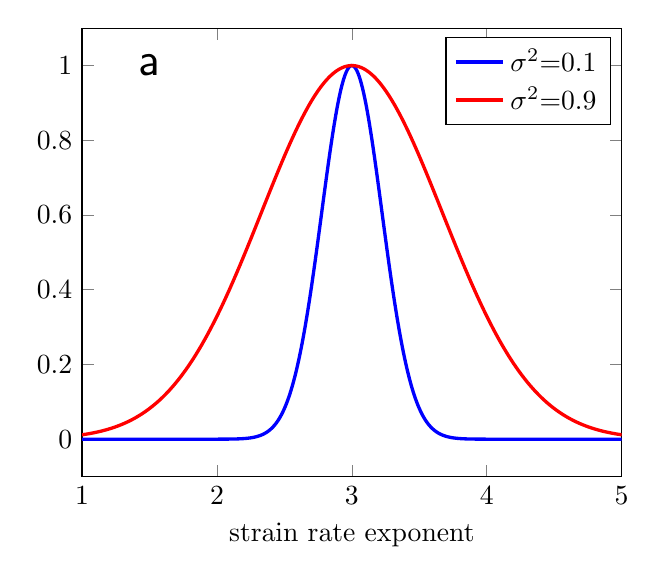
\begin{tikzpicture} 
\begin{axis}[ xlabel=strain rate exponent,xmin=1.0, xmax=5.0 ] % invoke external gnuplot as % calculator: 
  \addplot [mark=none,very thick, blue, samples=1000]{exp(-(x-3.0)^2/0.1)}; 
  \addlegendentry{$\sigma^2$=0.1}
  \addplot [mark=none,very thick, red, samples=1000]{exp(-(x-3.0)^2/0.9)}; 
  \addlegendentry{$\sigma^2$=0.9}
\node[font=\fontsize{18}{18}\sffamily] at (axis cs:1.5,1.0){a};

\end{axis} 
\end{tikzpicture}
}
\hspace{-0.2cm}\subfigure{

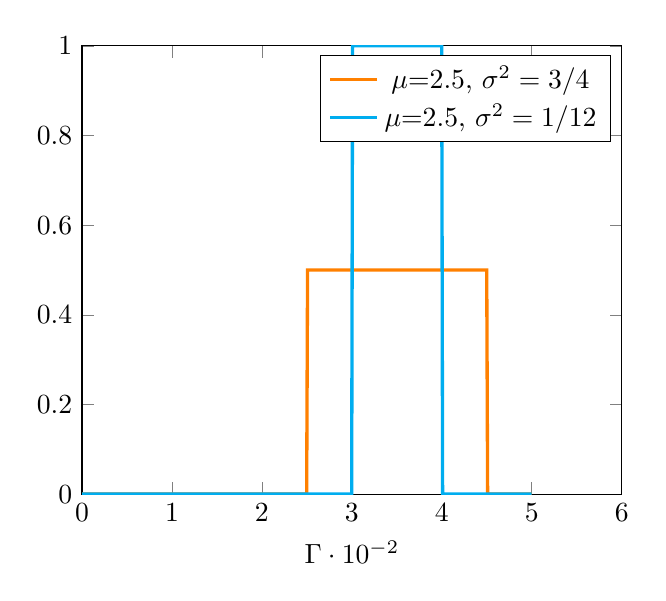
\begin{tikzpicture}[
    declare function={unipdf(\x,\xl,\xu)= (\x>\xl)*(\x<\xu)*1/(\xu-\xl);}
]
\begin{axis}[xlabel = $\Gamma \cdot 10^{-2}$,
    samples=1000,
%    const plot mark mid,
    xmin = 0, xmax = 6,
    ymin=0,ymax=1
]
\addplot [very thick, orange] {unipdf(x,2.5,4.5)};
 \addlegendentry{$\mu$=2.5, $\sigma^2 = 3/4$}
\addplot [very thick, cyan] {unipdf(x,3,4)};
 \addlegendentry{$\mu$=2.5,  $\sigma^2 = 1/12$}
%\node[font=\fontsize{18}{18}\sffamily] at (axis cs:1,0.9){b};
\end{axis}
\end{tikzpicture}

}

\caption{\mgnote{Right Subfigure still needs n a 'b'.}(a) Normal distributions for the strain rate exponent prior (b) Uniform distributions for the strain rate exponent prior. In (a) we compare the possibility of using two different normal distributions to demonstrate our knowledge or lack thereof of what the values of the strain rate exponent should be. }
\label{fig:prior_ex} 
\end{figure}

 Another possibility for a prior distribution is using a \textit{non-informative prior} \citep{Tarantola05}. A non-informative prior gives equal likelihood (equal probability) to each value such that no preference is given to a single value. Using non-informative priors can be advantageous when it is not apparent what an acceptable value is for a parameterized quantity, such as the strength of a weak factor An example of a non-informative prior is the uniform distribution in Fig.\ref{fig:prior_ex}b for the strain rate exponent. A uniform distribution has the following properties,
\begin{align}
\mathcal{U}(a,b) =
\begin{cases}
 \frac{1}{b-a}   &b\geq x \geq a \\
               0 &\quad \text{otherwise} \\
\end{cases}
\end{align}
with a mean and variance of 
\begin{align}
\begin{split}
\mu(a,b) &=\frac{1}{2}(a+b) \\
\sigma^2(a,b) &=\frac{1}{12}(b-a)^2 .\ \\
\end{split}
\end{align}

The uniform distribution in Fig.~\ref{fig:prior_ex}b has the same mean; however the variance is different. Compared to a normal distribution, the variance for the uniform distribution is determined by the range of likely values, each of which has the same probability.


 For a prior that is described by a normal distribution the mean $\mu$ and covariance, $\mathcal{C}$ is needed.
\begin{equation}
\ppi_{prior} = \mathcal{N}(\mu,\mathcal{C})
\end{equation}
Taking the negative log of the prior distribution results in a weighted misfit,
\begin{equation}
\mathcal{J}_{prior} = \frac{1}{2}(\mm-\mm_{mean})^T\mathcal{C}^{-1}(\mm-\mm_{mean})
\end{equation}
Therefore, the cost function would be
\begin{equation}
\begin{split}
  \mathcal{J}(\uu,\mm,p)&:= \frac{1}{2}\int_{\partial \Omega_1} (\mathcal{O}\uu-\uu_{\text{obs}})^T\mathcal{C}^{-1}_{vel}(\mathcal{O}\uu-\uu_{\text{obs}})d\partial\Omega_1 \\
%  &+\frac{1}{2}(\eta_0 - \text{exp}({\int_{\Omega_i} \ln \eta}))^{2} \\
   &+(\eta_0 - \text{exp}({\int_{\Omega_i} \ln \eta}))^{2} +\frac{1}{2}(\mm-\mm_{mean})^T\mathcal{C}^{-1}(\mm-\mm_{mean}).
\end{split}
\end{equation}
While the solution to the adjoint equation does not change, the gradient term for each parameter is modified,
\begin{equation}
\mathcal G:= \int_{\Omega} 2 \eta_{,i}(\IIinv, \Gamma, n, \sigma_y)\strain(\uu):\strain(\vv) d\Omega  + \mathcal{C}^{-1}(\mm-\mm_{mean})\mm_i.\
\end{equation}

These new gradients will be used to update the parameters as they measure the sensitivity of a parameter to an observation.

\section{Model Setup}
We have constructed a set of model constraints based on global observations. There are four components of these constraints: a global temperature distribution, the geometry of faults, the kinematics of plate motion, and the geometry and bounds on the effective viscosity within selected regions.

The temperature model has been constructed globally in a spherical shell from which  selected cross-sections are taken. The temperature of oceanic lithosphere follows a half-space cooling model using  updates to the digital grid of the age of the oceanic plates \citep{muller1997digital}.  
A thermal age was also used within continental regions with the following three regions: Cratons (300 Ma), areas near subduction zones (75 Ma), and other areas (200 Ma), as detailed in \citep{Stadler27082010}.
The thermal structure of slabs were constructed as follows. 
Initially the top surface of the slabs was based on the Slabs 1.0 surface which was based on detailed seismic constraints, including seismicity but also seismic reflection profiles \citep{Hayes2012}.
With normals pointing downward from this surface, an initial thermal structure of slabs based on the half space model using the age of the plate at the position of the trench was generated. This proceedure ensured continuity with the thermal structure of the oceanic lithosphere. Then we solved for thermal conduction at each depth over a duration equal to the travel time to reach the depth with the local convergence velocity (using the relative velocity vector). Although solved only with conduction, this procedure resulted in thermal structures close to those obtained in fully dynamic models. The tops of thermal  slabs were sharp in the corner of the mantle wedge and then progressively became more diffusive with depth.
Within the lower mantle the thermal structure was based on scaled tomographic models,
including a P-wave\citep{simmons2012llnl} and) a S-wave model \citep{ritsema1999complex}.
The lithosphere and upper mantle models and the upper and lower mantle were blended together as shown in the cross sections in \mgnote{cit Figure 1}.
models at 75 km and 550 km depths, respectively. We have used theseismo-tectonica approach for the shallower mantle and tomographically for the deeper as the seismic tomography models for slabs tend to be noisy.


On the surface of the earth we generated a veloctiy field from MORVEL56 \citep{GGGE2060} in a no net rotation (NNR) reference frame. Each cross-sectional model generally defines a great circle arc, with local unit vector \textbf{d} in the directon of the circle, such that we extracted the velocity $v_{xs}=\textbf{d}\cdot\textbf{v}$.  The NNR reference frame was used as the side-wals on the two-dimensionall cross sections preclude any large-scale differential motion between the bulk of thje mantle and the plates.

\begin{figure}[H]
\centering
\scalebox{0.9}{
\hspace{-1.8cm}\subfigure[]{
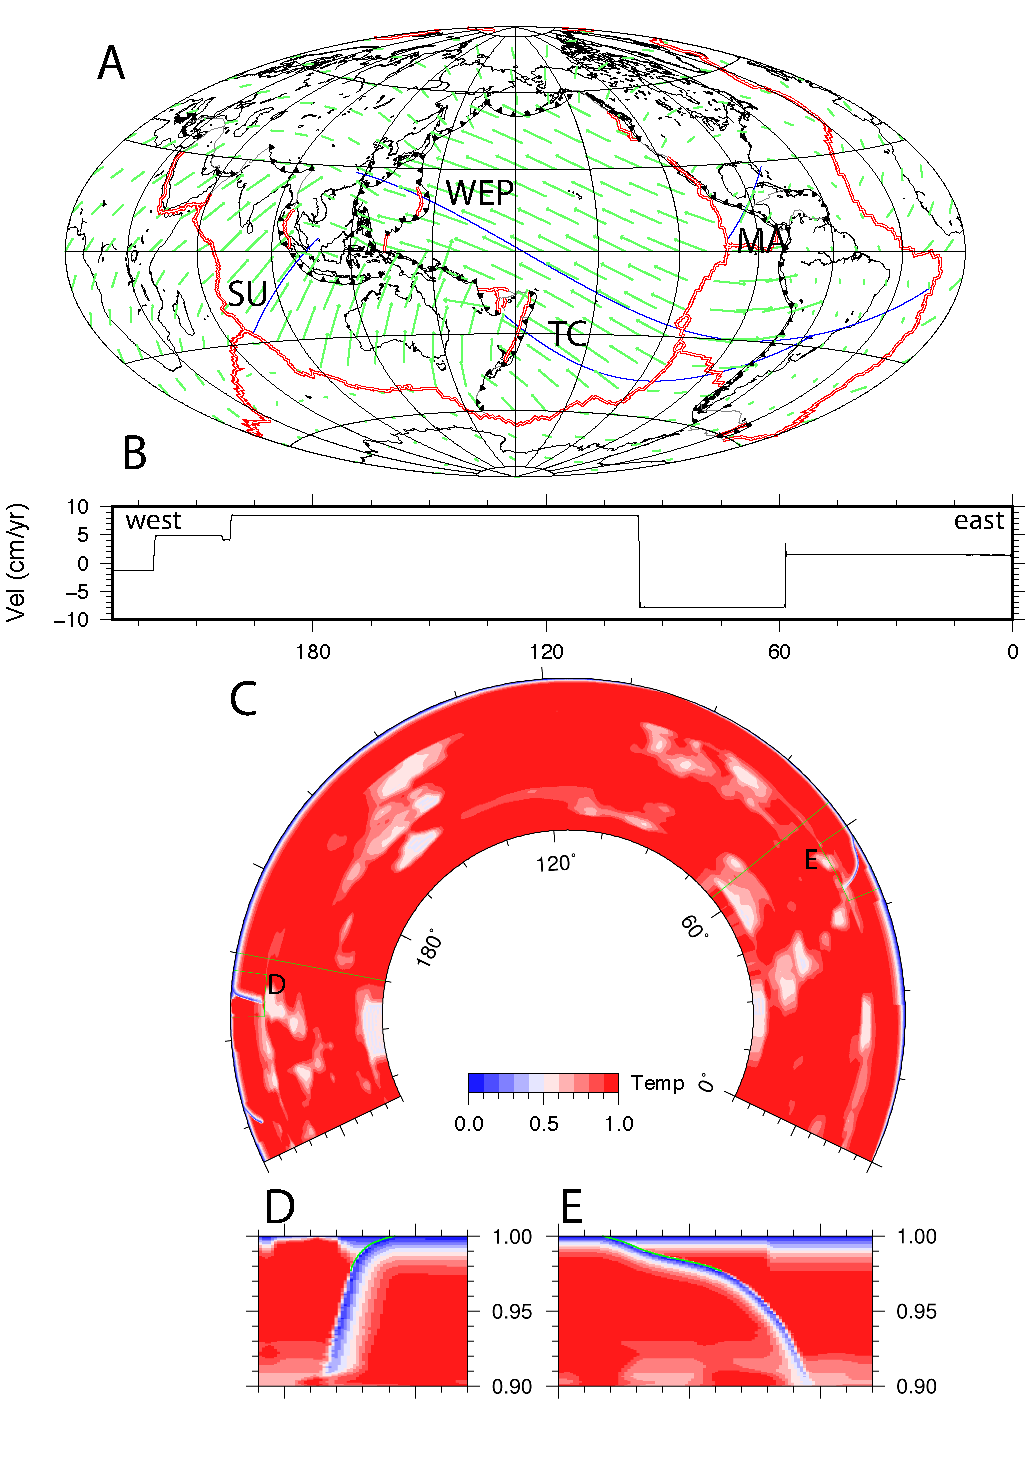
\includegraphics[height=150mm,width=100mm]{Summary_sections.pdf}%{mesh.pdf}
}

}
\caption{\mgnote{Make Figure Full page.} A. Velocity vectors in the no net rotation reference frame. Cross sections indicated with black lines, including wetsern to eastern Pacific (WEP), Sumatra (SU), Tonga to Chile (TC) and Middle America (MA) B. Velocity in the diection of cross-section WEP.(C)Temperature distribution for cross section WEP. Zoom in of the Marianas (in D) and the Chilean (in E) slabs for the WEP cross section. In D and E, the sloid green lines show the position of the weak zones.}
\label{fig:xsection2sumatra}
\end{figure}

Selecting a set of representative cross-sections in which all of the driving forces may be partially represented as two-dimensioanlly proved to be quite difficult, as it is likely that not plate and subduction zone is truely two-dimensional. 
Nevertheless, we have chosen a set of cross-section in which plate motion was generally orthognonaly to the strike of the trench and which represent some of the end-member cases of what is considered to be from the least to the most seismically coupled subduction zones (Fig.\mgnote{REF}). To investigate the coupling for various seismically coupled subduction zones, we consider the cross-sections in Fig. \ref{fig:xsection2sumatra}. Our primary cross-section is the largest dimension and contains three subduction zones that span the range from the seismically coupled (Chile) to least coupled (Marianas). This cross section contains one subduction zone with back-arc extension. The cross-sections in Fig.\ref{fig:xsection2sumatra}b,c are smaller than in  Fig.\ref{fig:xsection2sumatra}a, and thus do not contain the coupling variability of the larger cross-section; however those cross-sections represent other subduction zones that exhibit substantial coupling (Sumatra) and very little coupling (Tonga).

\begin{table}[H]
  \caption{\mgnote{Are these values acrually used?}Summary of seismic coupling coefficients ($\kappa_s$) is the seismic coupling coefficient, while $\chi_g$ is the geodetic coupling coefficient \citep{scholz2012seismic}.} % title of Table
  \centering  % used for centering table
  \begin{tabular}{c c c} % centered columns (2 columns)
    \hline \hline                        %inserts double horizontal lines
    Subduction Zone & $\chi_s$ & $\chi_g$  \\ [0.5ex] % inserts table
    %heading
    \hline                  % inserts single horizontal line
    North Tonga  &0.65 &N/A   \\
    Central Peru &0.8 &0.75 \\
    South Peru &0.75 &N/A \\
    Central Chile &0.70 &1.0 \\
    South Chile  &0.82-1.0 &0.96 \\
    North Chile &0.94 &1.0 \\
    Sumatra &0.5-0.83 &1.0 \\
    \hline %inserts single line
  \end{tabular}
  \label{table:parameters} % is used to refer this table in the text
\end{table}


The fault zone decoupling between converging plates at subduction zones, generally thought to be the places on which great earthquakes occur, were represented as weak zones with unknown viscosity. Weak zone factor, created by a stencil with a center line defined by the Slabs 1.0 surface \citep{Hayes2012}, was defined as
\begin{equation}
\Gamma_{stencil} = 1.0 - (1-\Gamma_i)\exp\{-(d_i-d_0)^2/(2\sigma_{smooth}^2)\}
\end{equation}
and with coefficient $\Gamma_i$ that was recovered in ~\eqref{eq:rheo}, $d_0$ is the center-line profile, $\sigma_{smooth}$ is the amount of smoothing for the weak zone.
 For our models, we assume the values of (mantle parameters) which are summarized in Table ~\ref{table:parameters}.

\begin{table}[H]
  \caption{Assumed parameters left as constants in the }
  \centering  % used for centering table
  \begin{tabular}{c c c} % centered columns (2 columns)
    \hline \hline                        %inserts double horizontal lines
    Symbol & Parameter & Value  \\ [0.5ex] % inserts table
    %heading
    \hline                  % inserts single horizontal line
    $\rho$ & Density ($\rho$)  & 3300 kg/m$^3$ \\
    $g$ & Gravity ($g$) & 9.81 m/s$^2$ \\
    $\alpha$ & Coefficient of Thermal expansion ($\alpha$) & 2 $\times$ $10^{-5}$ \\ 
    $\Delta T$& Temperature Difference $\Delta T$ & 1400 K \\
    $D$& Depth of layer ($D$) & 1500 km \\
    $\kappa$& Thermal Diffusivity ($\kappa$) & $10^{-6}$  m$^2$/s \\
    $\eta_{\text{ref}}$& Reference Viscosity  ($\eta_{\text{ref}}$) & $10^{20}$ Pa $\cdot$ s \\
    Ra & Rayleigh Number (Ra) & 2.92 $\times$ $10^9$ \\
    $n$ & Strain rate exponent in lower mantle ($n$) & 1.0 \\
    \hline %inserts single line
  \end{tabular}
  \label{table:parameters} % is used to refer this table in the text
\end{table}

\mgnote{This needs to be rewritten. Are these data (tomography and plate model actually varied? In then end, I don't thoink so}These cross-section optimizations have uncertainties in not only plate motions, but in the tomography model used in the lower mantle, as there are different tomography models S40RTs or \citep{simmons2012llnl}), which in turn can possibly influence the inference of the global parameters (strain rate exponent and yield stress). Furthermore, plate motion data is highly dependent on the reference frame used such as hotspots, one fixed to a specific plate (Pacific for example), or the no-net-rotation(NNR) reference frame. In addition to the uncertainty of the reference frame, there is uncertainty in the Euler pole (latitude and longitude) of each plate along with the rotation (degrees/Ma) which can possibly influence the parameter estimation of plate couplings.


\mgnote{This is vague. The viscosity constraints need to be described in precise terms (e.g. magnetide of visocisty and geometry with reference citations}As presented earlier, the average effective viscosity data is an additional constraint that we will explore to determine the effect it has on the inference of the the rheological parameters. It is posited that since the effective viscosity is an observation from the mantle, then this data should better constraint on the global parameters such as the strain rate exponent, activation energy, and upper mantle prefactors. We will place the average effective viscosity constraint under the South American plate, as it is the only plate in our models with a substantial continental plate overriding a subduction zone.

\section{Results}

\mgnote{Both of these sub-sections suffer from the same problem. You say we tried case x and we get y, but there is essentially no discussion of the 'why'. This is geodynamics, we are in the business of providing answers on the 'why'. How can you arrive at these concluions and discussions. You need to look at the equations, both of motion and  vicosity, perhaps plost of effective viscosity and then your condition distrbutions. I will give a lot of commentary in the days ahead on improving in this regard. Getting plots to use on Effective Vistory in cross sections would be really helpful.}

\subsection{Inversions}
From the optimization we infer plate coupling across subduction zones and global parameters such as the yield stress and strain rate exponent. 
By first focussing on a single large cross-section (WEP), the strengths and limitations of the optimization method are explored (Fig.\ref{fig:xsection2sumatra}a).  
For the inversion, guesses for the rheological parameters and coupling coefficients are required for the initial forward model. \mgnote{is this wise; shouldn't one model explore using larger and smaller values in addition to the normal guess?}In all models, we choose an initial weak zone factor of $\Gamma=10^{-5}$, which typically decouples the plate boundaries allowing subduction. \mgnote{Is this also the only guess that you use?}We choose an initial guess of 125 MPa for the yield stress because it provides a reasonable amount of dynamic weakening in forward models while satisfying estimates from seismicity \citep{craig2014reassessment}, while using an initial strain rate exponent of $n=3.0$, a value typically associated with mantle convection and within the bounds imposed from laboratory experiments \citep{ranalli1995rheology}, an activation energy $E_a=203.6$kJ/mol, a value we found through multiple forward models in which plates are sufficiently strong to act as stress guides. %We set up a reference case with 
%the strain rate exponent, yield stress and plate boundary couplings, and the upper mantle prefactor as unknowns.  
 %Furthermore, we choose to infer the radial prefactor of the upper mantle, a parameter that controls the effective viscosity of the upper mantle.  


\begin{sidewaystable}

\centering

	\begin{table}[H]
		\caption{Case study summary\mgnote{We will need a complete list of cases and this is not comprehensive enough. As We read and discuss we should be able to fill this up. Also for the Collumns in which a parameter is set to a fixed value, like $E_a$ give the value and and underline to signify that it was fixed.}} % title of Table
		\centering  % used for centering table
		\begin{tabular}{c c c c c c c c  } % centered columns (2 columns)
		\hline \hline                        %inserts double horizontal lines
		Case & Subduction Zone & \textit{n} &$\sigma_y$&$\Gamma$ (SAM/RYU/IZU) $\cdot 10^{-5}$ &UM Prefactor &$E_a (kJ/mol)$&Visc. data   \\ [0.5ex] % inserts table
		%heading
		\hline                  % inserts single horizontal line
	      	 1 &Complete& 3.042 & 148 & $100/0.82/0.77$ &  4700& no & no  \\
	        2 &Complete& 3.046 & 146 & $67.3/0.773/0.798$ & no & no & no \\
	        3 &Complete& 3.08 & 141.8 & $87.3/0.703/0.7448$ & no & yes & no \\
	        4 &Complete& 3.0225 & 155 & $94.6/0.8423/0.889$ & no & & no (priors used) \\
                5 &Sumatra& 3.048 & 143.1 & $63.9$ &  assumed& assumed& no \\

                 6 &Sumatra& 3.1 & 120 (assumed) & 44.1 & no & 207.2   &no\\
                  7 &Sumatra& 3.0 (assumed) & 128.1 & 38.2 & no & 190.7   &no\\
              8 &Tonga  & 3.0621 & 139.1 & 2.21& no & no &no  \\              
               9 &Tonga  & 3.051 & 135.2 & 0.7& assumed & 186.2 &no  \\             
              10 &Tonga  & 3.087 &  120 (assumed) & 0.71 &assumed &175.6  &no  \\              
               11 &Tonga  & 3.0 (assumed) & 127.7 & 0.8 &assumed &198  &no  \\             
               12 &Central America  & 3.0621 & 139.1 & 2.21& assumed & assumed &no  \\             
                 13 &Central America  & 3.12 & 120 (assumed) & 6.3& assumed & 178.1 &no  \\         
                 14 &Central America  & 3.0 (assumed) & 132.1 & 0.84& assumed& 207.2 &no  \\        
          
          
                \hline %inserts single line
		\end{tabular}
		\label{table:inversions} % is used to refer this table in the text
		\end{table}
\end{sidewaystable}





%We use this cross-section as the surface velcoities are almost-parallel the the great-circle. The length of this arc is approximately, 25,410 km.
For the WEP cross-section, we ran a suite of inversions where we varied the parameters to be inferred as given in Table \ref{table:inversions}.  We first inferred the plate couplings, strain rate exponent, yield stress and upper mantle prefactor as shown in Case 1 and Fig.\ref{fig:inverse1} so as to see if there are variations in mechanical coupling as seen from seismic coupling. The effective viscosity in Case 1 (Fig.\ref{fig:inverse1}a) shows a weak upper mantle in addition to dynamic weakening in hinge zones.  In Case 1, we were able to infer the plate couplings within 5 adjoint iterations (Fig.\ref{fig:inverse1}b), and furthermore find that the inferred couplings for South America, Izu-Bonin and Ryukyu are different Fig.\ref{fig:inverse1}b (filled circles).The inferred strain rate exponent is slightly greater than 3.0 (initial guess), though still within the bounds provided by experiments, while the inferred yield stress is 148 MPa. An important question about Case 1 is if these values would change if we chose a different initial guess for one of the inferred parameters. Using different initial guesses for the strain rate exponent, as shown in Table \ref{table:initial_guess}, we find that we are able to recover similar values for the plate couplings, strain rate exponent and yield stress. Furthermore, we find a similar trend that the plate couplings for the three subduction zones are different, while they still retain the the same relative ordering of plate coupling.   
%The relative ordering of inferred plate couplings in Case 1 strongly suggests that the inferred coupling may lend credence to the notion that the Nazca-South America plate boundary is more coupled compared to Ryukyu and Izu-Bonin plate margins.
A new parameter that is included in the inversion for Case 1 is the upper mantle prefactor, which plays an important part in controlling the effective viscosity,(increasing this prefactor would increase the effective viscosity), and the amount of shear thinning in the upper mantle. We find that we are able to infer the upper mantle prefactor within 5 adjoint iterations, thus demonstrating that this parameter can be inferred within a reasonable amount of iterations.


	
While we explored the influence of the global parameters and plate couplings with the additional upper mantle prefactor parameter, it would important to see if there is any change to the ordering of the plate couplings by just inferring the yield stress and strain rate exponent with those couplings. We do so in Case 2 by  by keeping the upper mantle prefactor fixed, effectively conditioning on the upper mantle pre-factor (similarly done in \citep{ratnaswamy2015adjoint}). In this case, we find that the inferred strain rate exponent is 3.042, which is close to the initial guess of 3.0, (similar to Case 1) and is only $\approx$ 0.1\% larger than the inferred strain rate exponent in Case 1. Similar to the strain rate exponent, the inferred yield stress in Case 2 is 146 MPa, only $\approx$1\% lower than the inferred yield stress in Case 1, while the inferred plate couplings follow the same pattern as the least coupled subduction zones are Ryukyu and Izu-Bonin. We see in Fig.\ref{fig:inverse1}a, that we not only recover different plate couplings for the three subduction zones but that their relative ordering is the same as in Case 1, possibly suggesting that the physics of these mantle flow models prefer this relative plate coupling ordering. 

\begin{table}[H]
		\caption{Sensitivity of initial guesses for Case 1} % title of Table
		\centering  % used for centering table
		\begin{tabular}{ c c c } % centered columns (2 columns)
		\hline \hline                        %inserts double horizontal lines
		 \textit{n} &$\sigma_y$&$\Gamma $(SAM/RYU/IZU) $\cdot 10^{-5}$   \\ [0.5ex] % inserts table
		%heading
		\hline                  % inserts single horizontal line
	         2.95/3.042 & 148 & $100/0.82/0.77$    \\
	         2.98/3.046 & 146 & $67.3/0.773/0.798$  \\
	        2.97/3.0225 & 141.8 & $87.3/0.703/0.7448$  \\             
                \hline %inserts single line
		\end{tabular}
		\label{table:initial_guess} % is used to refer this table in the text
		\end{table}


Now that we can infer the rheological parameters of this cross-sectional model, we turn our attention to better estimate those parameters by using the average effective viscosity, while investigating if there is any change to the relative plate coupling for these subduction zones.  We find in Case 3 using both the average 
effective viscosity below South America and plate motions that the strain rate exponent is 3.08, which is larger than the inferred strain rate exponent in Cases 1 and 2, implying an increase in shear thinning, which would cause an increase in plate motion. The inferred yield stress for Case 3 is 141.8 MPa which is quite similar to the inferred yield stress from Cases 1 and 2 and would result in a similar amount of dynamic weakening at the hinge zones. Similar to Cases 1 and 2, we find that there is a preferred coupling for each subduction zone, such that the Nazca-South America subduction zone is the most coupled, (approximately an order of magnitude more), compared to Izu-Bonin and Ryukyu subduction zones, which seemingly suggests that regardless of the inferred global parameters, there is a preferred ordering of the mechanical coupling.
  % The first case study is shown below in Fig.\ref{fig:inverse1}
\begin{figure}[H]
\centering
%\hspace{-0.2cm}\subfigure[]{
%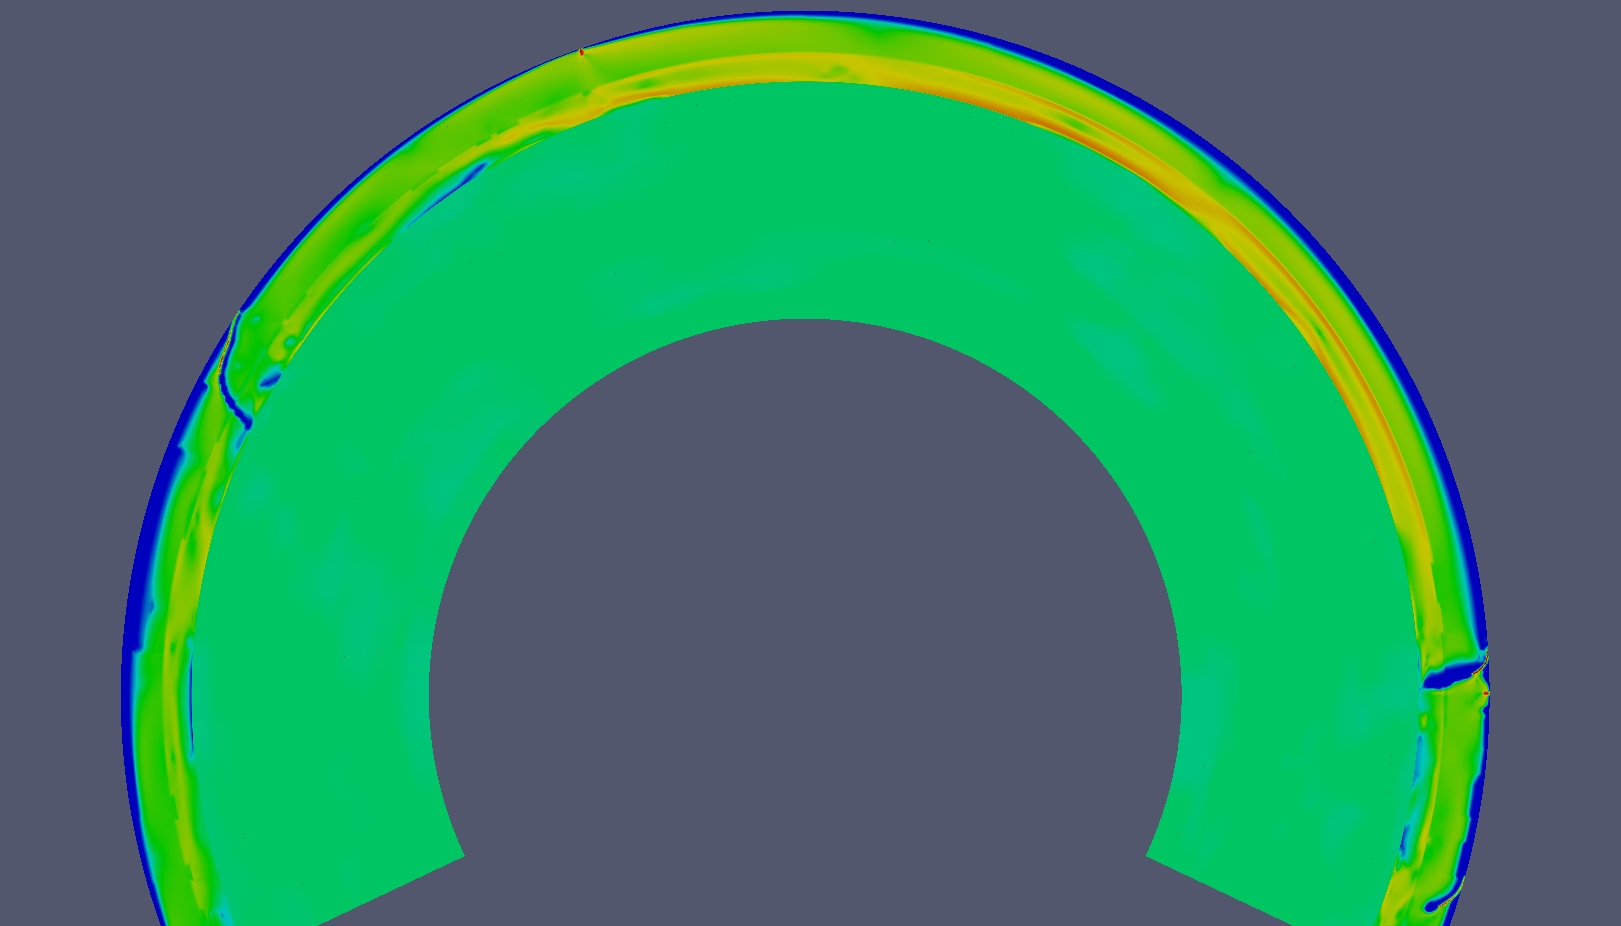
\includegraphics[height=65mm,width=128mm]{visc_no_stress.jpg}%{mesh.pdf}
%}
\hspace{-0.85cm}\subfigure[]{
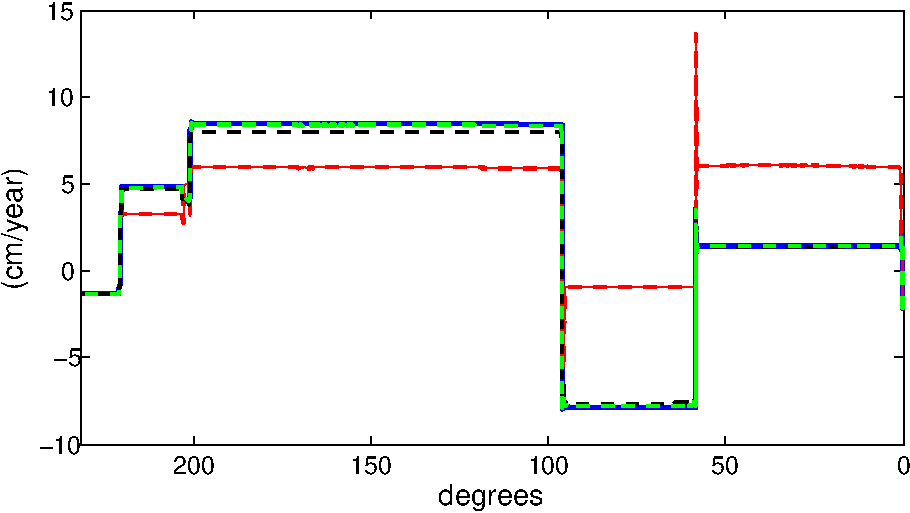
\includegraphics[height=35mm,width=68mm]{data_vel.pdf}%{mesh.pdf}
}
\hspace{-0.2cm}\subfigure[]{
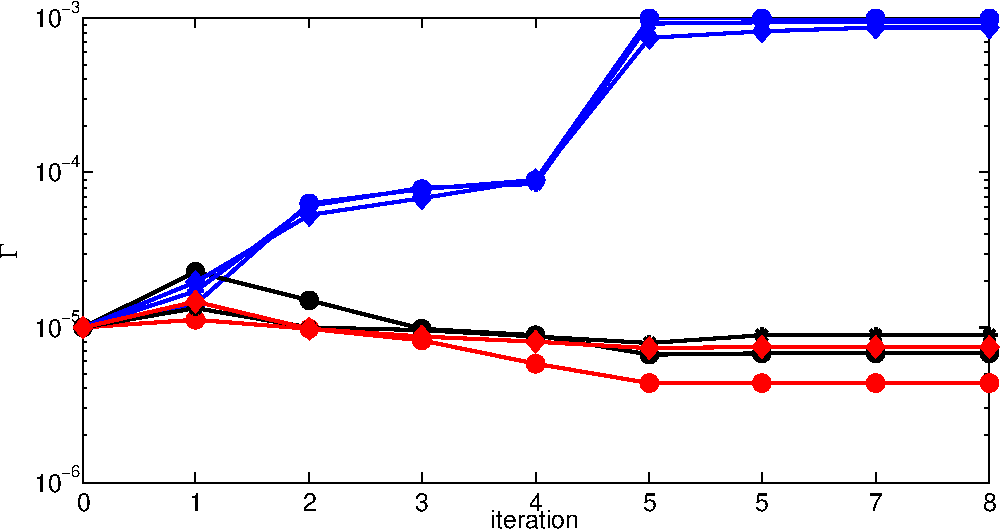
\includegraphics[height=35mm,width=58mm]{paper_gamma2.pdf}%{mesh.pdf}
}
\hspace{-0.2cm}\subfigure[]{
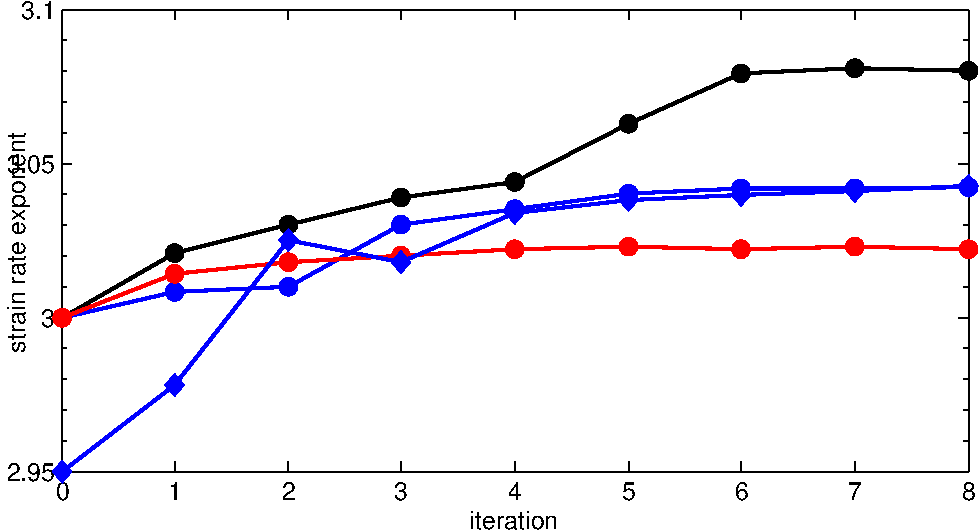
\includegraphics[height=35mm,width=58mm]{paper_strain2.pdf}%{mesh.pdf}
}
\hspace{-0.2cm}\subfigure[]{
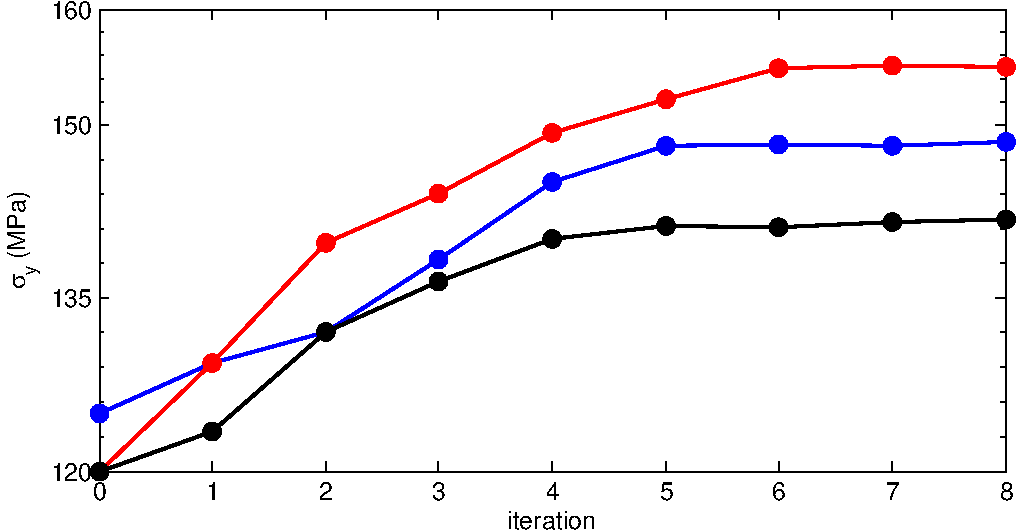
\includegraphics[height=35mm,width=58mm]{paper_yield2.pdf}%{mesh.pdf}
}
%\hspace{-0.2cm}\subfigure[]{
%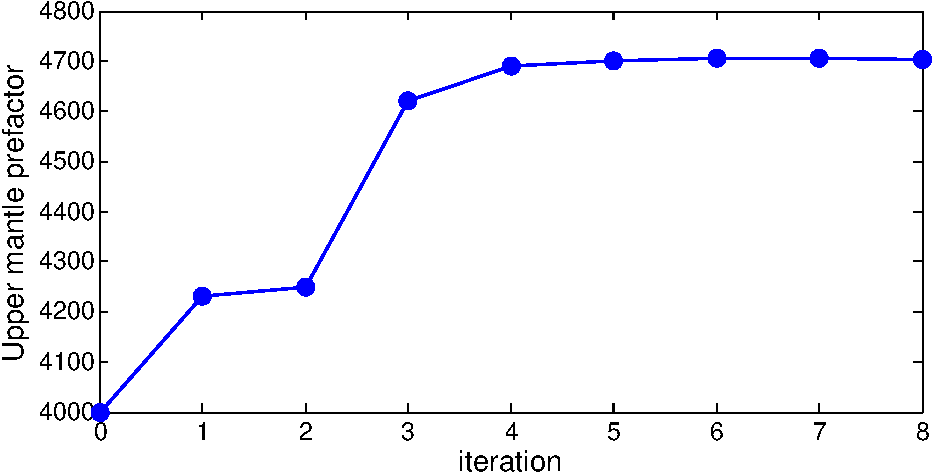
\includegraphics[height=35mm,width=58mm]{um_chap4.pdf}%{mesh.pdf}
%}
\caption{\mgnote{Here are some general comments about these kinds of Figures. Please carve these comments out and take them very seriously. First. The "a", "b", etc., should be inside the Figure. Using LaTeX to this creates messy Figures that are hard to work with. This is easy in Adobe Illustrator. Having a hanging block by shifting from two collumns to one collumn is a waste of space and awkard looking. Also, learn how to use MatLab to makin better sub-figures if that is what you are going to do. You only have 'major labled tick marks'; you should youse fewer labels and more sub-tick marks.}(a) i\mgnote{ panels b-e are a waste of space and not informative for the reader because you are only showing the convergence of three models. I would ponetially show the convergence of 4 models. 1. The model you have shown. 2. a model with a differnt IC guess. 3. What happends when you use Vel+effective viscosity constraint (new to this paper). 4. What happens hen you use Vel+priors. Does this speed up convergence? Given different convergence speeds. }Surface velocity comparison between data and different iterations (Case 1).(b)Plate boundary weakfactor iteration (South America (blue lines), Izu-Bonin (red lines), Ryukyu (black lines), with \textit{circles} being velocity data only, \textit{diamonds} being velocity and effective viscosity data and \textit{asterisks} being velocity and priors  (c) strain rate exponent iteration \textit{blue circle} being plate velocities, \textit{blue diamonds} being a different initial guess, \textit{black circle} being velocity and effective viscosity data and \textit{red circle} being velocity and priors (d) yield stress iteration with \textit{blue circle} being plate velocities, \textit{black circle} being velocity and effective viscosity data and \textit{red circle} being velocity and priors .}
\label{fig:inverse1}
\end{figure}

While using additional data may reduce the uncertainty of the inferred parameters, the inclusion of prior knowledge would certainly aid in reducing the variance of the inferred parameters. Using knowledge from experimental data \citep{korenaga2008new}, we include prior knowledge as Gaussian distributions with mean values of $\overline{n}=2.95$,$\overline{\sigma}_y = 120 MPa, \overline{\Gamma}=10^{-5}$, while using variances that do not place strong constraints on the inferred parameters (Case 4). 
 With prior knowledge, we find that the order of plate couplings corresponds to what was found from cases 1-3. Furthermore, the recovered strain rate exponent is slightly smaller (3.0225) , while the yield stress is slightly larger (155 MPa), than Cases 1-3. It is important to note that the inferred parameters obtained from using priors are similar to values inferred when priors are not used, suggesting that the underlying physics strongly prefers certain values of the global rheological parameters and a particular relative ordering of plate couplings.

While the larger cross-section (Cases 1-4) has the advantage of having subduction zones of varying seismogenic coupling, it is important to compare the parameter inferences from the larger cross-section to smaller cross-sections to determine if the global parameters would be of similar magnitude and how. The Sumatra subduction zone is of particular interest as it is thought to be one of the more seismically coupled subduction zones. Therefore, we repeat similar case studies for the Sumatra subduction zone.

 % The first case study is shown below in Fig.\ref{fig:inverse1}
\begin{figure}[H]
\centering
%\hspace{-0.2cm}\subfigure[]{
%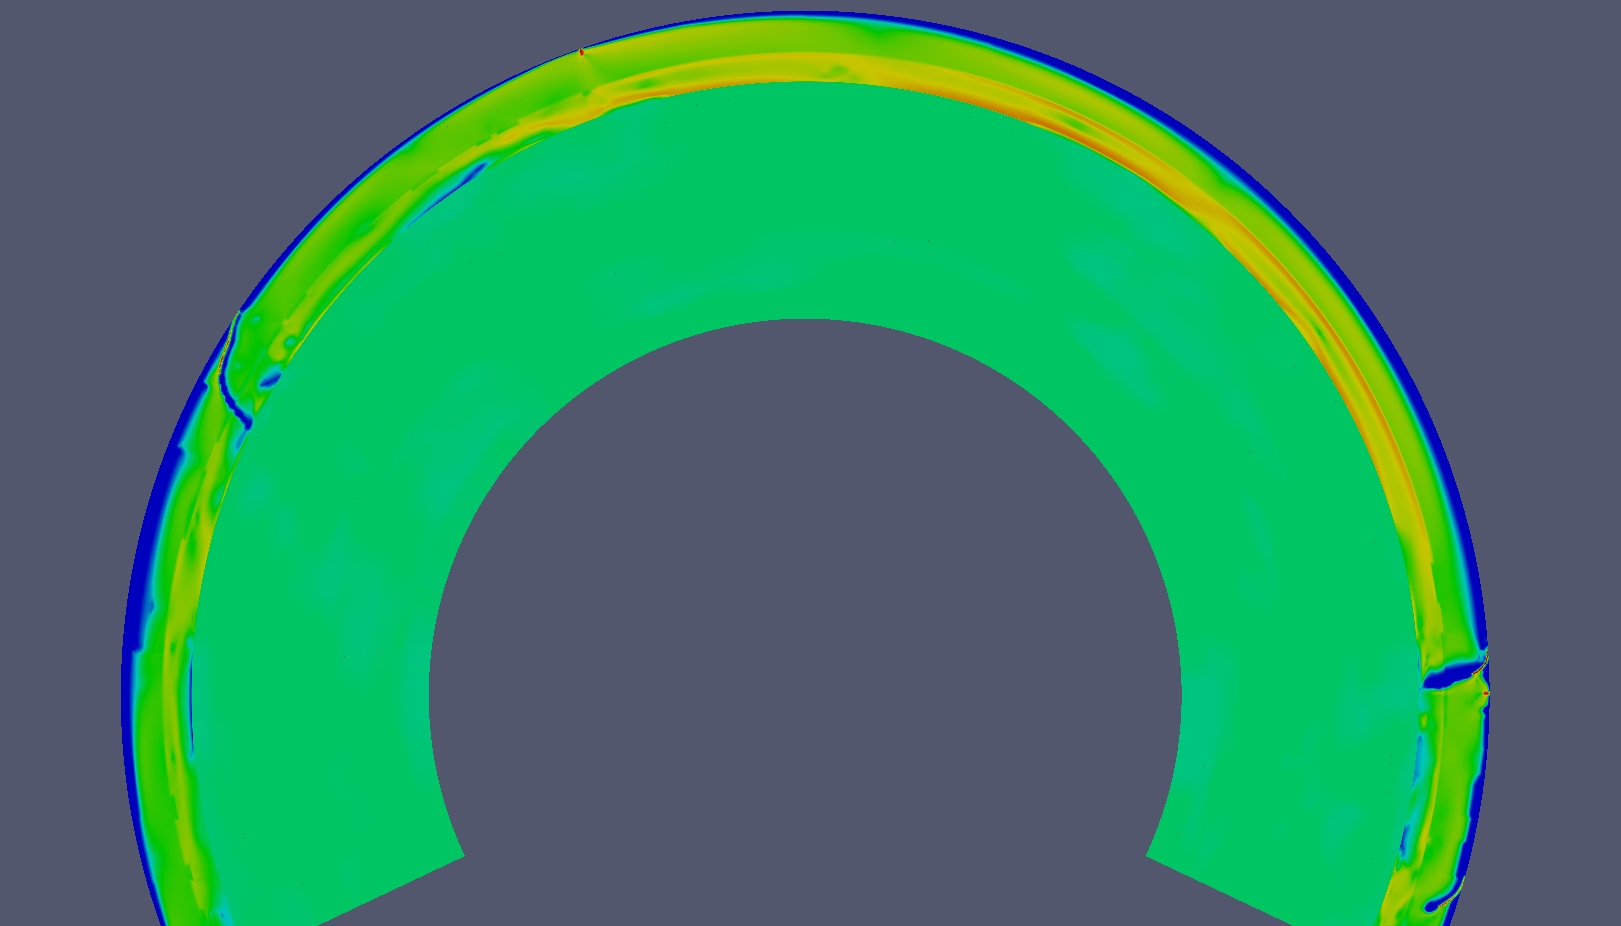
\includegraphics[height=65mm,width=128mm]{visc_no_stress.jpg}%{mesh.pdf}
%}
\hspace{-0.85cm}\subfigure[]{
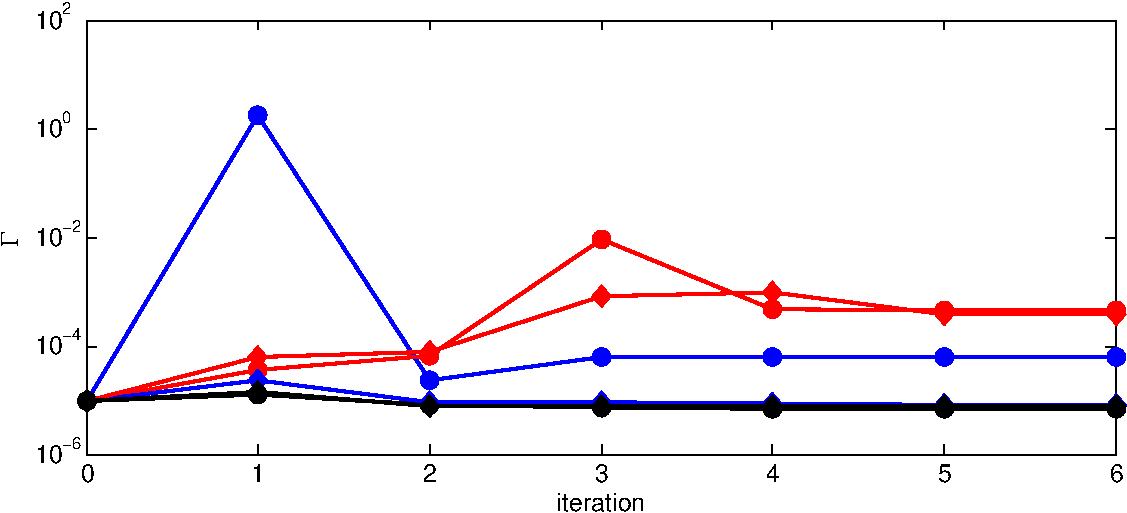
\includegraphics[height=35mm,width=68mm]{paper_gamma1.pdf}%{mesh.pdf}
}
\hspace{-0.2cm}\subfigure[]{
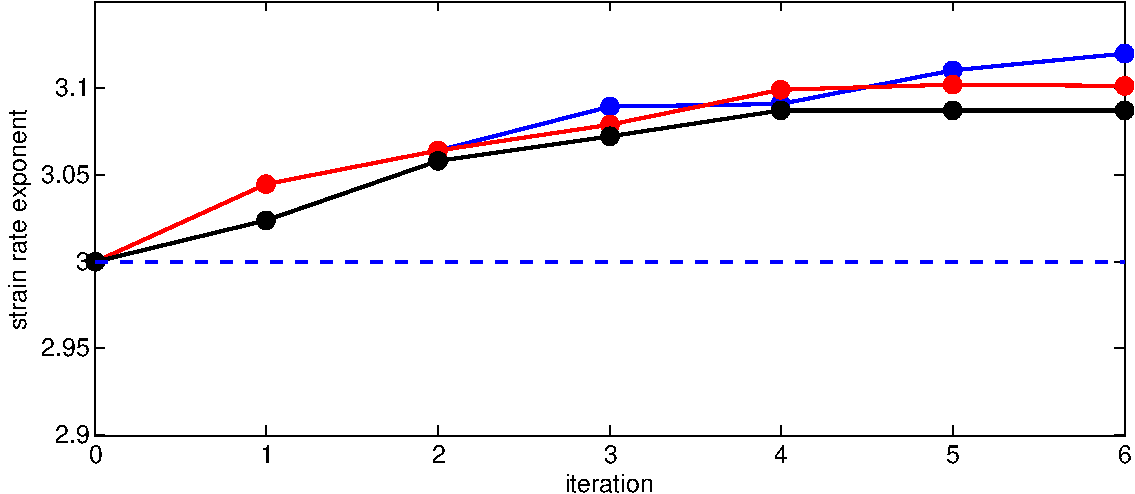
\includegraphics[height=35mm,width=58mm]{paper_strain1.pdf}%{mesh.pdf}
}
\hspace{-0.2cm}\subfigure[]{
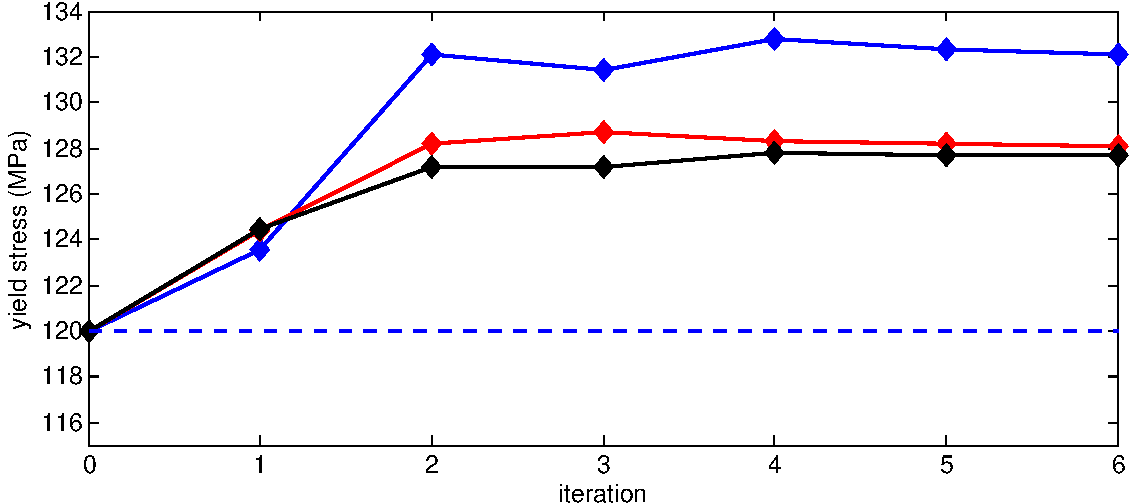
\includegraphics[height=35mm,width=58mm]{paper_yield1.pdf}%{mesh.pdf}
}
\hspace{-0.2cm}\subfigure[]{
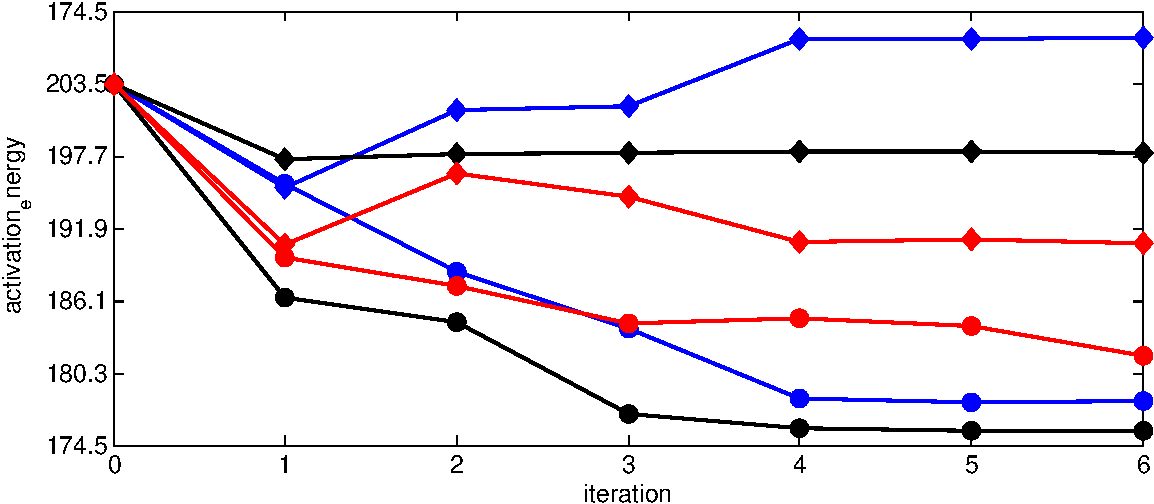
\includegraphics[height=35mm,width=58mm]{paper_activ1.pdf}%{mesh.pdf}
}
%\hspace{-0.2cm}\subfigure[]{
%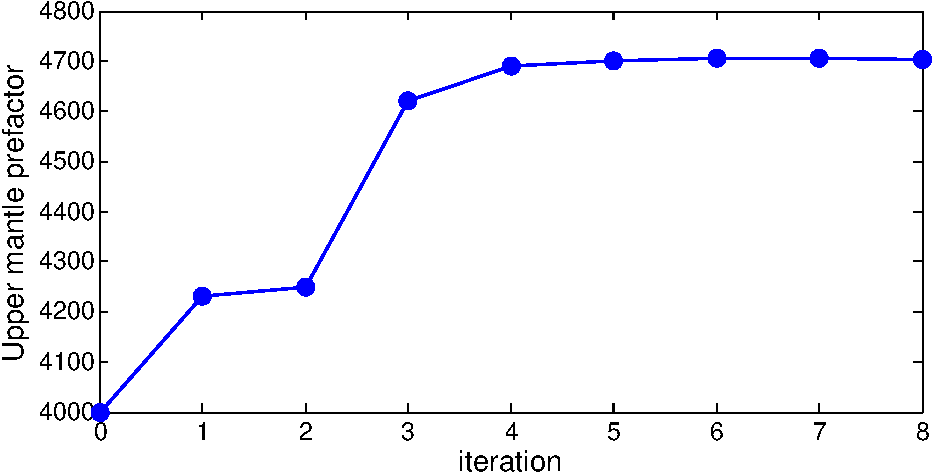
\includegraphics[height=35mm,width=58mm]{um_chap4.pdf}%{mesh.pdf}
%}
\caption{(a)Plate boundary weakfactor iteration (Central America (blue lines), Sumatra (red lines), Tonga (black lines). It should be noted \textit{diamonds} represent strain rate exponent held fixed, while \textit{circles} represent yield stress held fixed (c) strain rate exponent iteration, \textit{dashed line} represents the fixed value of yield stress (d) yield stress iteration \textit{dashed line} represents the fixed value of the strain rate exponent.}
\label{fig:inverse1}
\end{figure}
We find in Case 5, that the inferred the strain rate exponent is approximately 3.05, while the yield stress is approximately 143 MPa. The inferred plate coupling for Sumatra is larger than that of Ryukyu and Izu-Bonin in Cases 1-4, which seems to further suggest that mechanical coupling is independent of rheology. Plate coupling, yield stress and strain rate exponent are important to mantle flow models; however the activation energy is key when it comes to controlling the amount of temperature dependence there is within these models. To this end, we included the activation energy in our inferences in Case 6, and find that the inferred value is $207$ kJ/mol, while obtaining a larger coupling for Sumatra compared to what was found for Izu-Bonin and Ryukyu in  Cases 1-4. Furthermore, our inferred strain rate exponent and yield stress are similar to what we obtained in Case 5, suggesting that these parameters are preferred to produce the observed plate motions. 


While we are able to infer the global parameters and the activation energy, there is still is a question as to whether the plate coupling for Sumatra would change if we kept one of the global parameters fixed. To this end, we explored this question by fixing either the yield stress or strain rate exponent and inferring the plate coupling and activation energy in Cases 7-8. When the yield stress is fixed (Case 7), we find that there is a slight increase in the strain rate exponent, while the inferred plate coupling is still larger than Ryukyu and Izu-Bonin. Similarly, when the strain rate exponent is fixed (Case 8), the yield stress increases slightly from the initial guess, while the plate coupling for Sumatra is still larger compared to Izu-Bonin and Ryukyu. 

We similarly repeated the same types of case studies for Tonga (Cases 9-11) and Central America (Cases 12-14). We find that the plate couplings for Tonga and Central America are smaller than Sumatra (Central America being larger than Tonga) , regardless of which parameters we kept fixed. Furthermore find that the yield stress and strain rate exponent for both Tonga and Central America are of similar magnitude compared those that were obtained for Sumatra, further suggesting that there is a preferred yield stress and strain rate exponent for mantle flow models to match plate motions. The inferred activation energy for Tonga and Central America are different than that of Sumatra; however the difference in those values are not significant as there is a similar amount of temperature dependence in viscosity in all of these models partly due to the viscosity bounds in the rheological law.







\subsection*{Uncertainty Quantification for Plate boundary stresses}

An important part of our studies was to quantify the uncertainty of the inferred rheological parameters that was similarly done in \citep{ratnaswamy2015adjoint} by examining the posterior distributions, more specifically the conditional distributions. The conditional distributions convey not only the uncertainty in each parameter, but the trade-offs and how they contribute to the underlying physics of these models. In Fig.\ref{fig:distrib}a,b, we compare the conditional distributions for the plate couplings vs. yield stress and strain rate exponent in Case 1 and find that there is a clear demarcation between the least coupled subduction zones (Ryukyu and Izu-Bonin) and South America. The partitioning of the subduction zones suggest that the South America plate boundary is more mechanically coupled compared to Ryukyu and Izu-Bonin regardless of the global parameter (yield stress and strain rate exponent). Furthermore, we find a similar partitioning for Cases 2-3 for the larger cross-section, which seems to suggest that regardless of prior knowledge or average effective viscosity data being used in these inversions, there still is a preferential ordering with regards to plate coupling. 

An important consequence of these conditional distributions are the trade-offs between the rheological parameters that were previously found \citep{ratnaswamy2015adjoint}. We see that there exist strong positive correlations between the strain rate exponent and yield stress in Fig.\ref{fig:distrib}c, a negative correlation between the plate couplings and yield stress in Fig.\ref{fig:distrib}b and a positive correlation between plate couplings and strain rate exponent in Fig.\ref{fig:distrib}a that were previously observed in \citep{ratnaswamy2015adjoint}. The positive correlation between the strain rate exponent and yield stress suggests that as the strain rate exponent increases, plate motions increase, thereby resulting in an increase in yield stress in order to compensate for the increase in plate velocity. Likewise, the increase in plate coupling causes an increase in viscosity which reduces plate velocity.  To compensate for this increase in viscosity, a decrease in yield stress is needed, which causes weakening in plates, thereby increasing plate motion. Similarly, as plate coupling increases (increase in viscosity in the fault zone), an increase in the strain rate exponent is needed as compensate for the decrease in plate motion.  
%A new parameter that we included in our inferences is the upper mantle prefactor, a value that controls the effective viscosity in the upper (or lower) mantle. We find that there exists strong correlation between the upper mantle prefactor and strain rate exponent. This correlation is not surprising as the effective viscosity is highly dependent on the upper mantle prefactor and the strain rate exponent, i.e. an increase in strain rate exponent leads to more shear thinning (decrease in effective viscosity), which would give rise to an increase in the upper mantle prefactor.

\begin{figure}[H]
\centering
\hspace{-0.85cm}\subfigure[]{
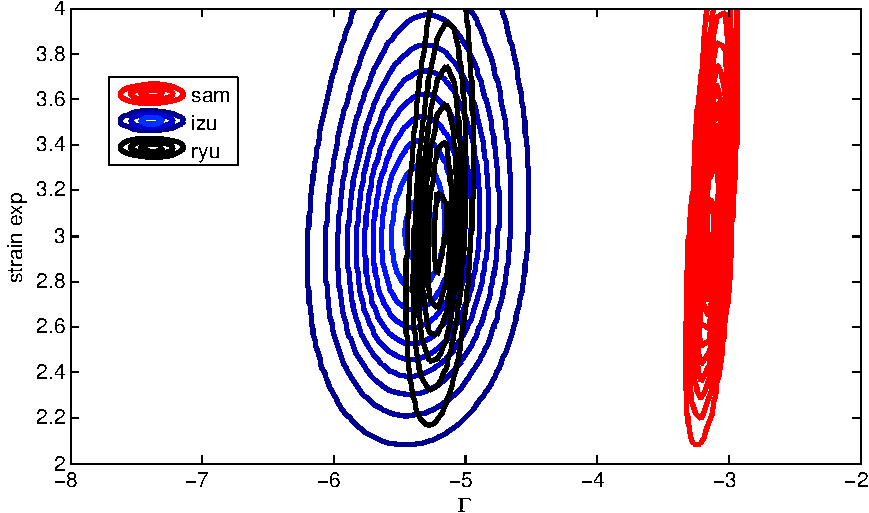
\includegraphics[height=35mm,width=52mm]{gauss_weak_strain.pdf}%{mesh.pdf}
}
\hspace{-0.1cm}\subfigure[]{
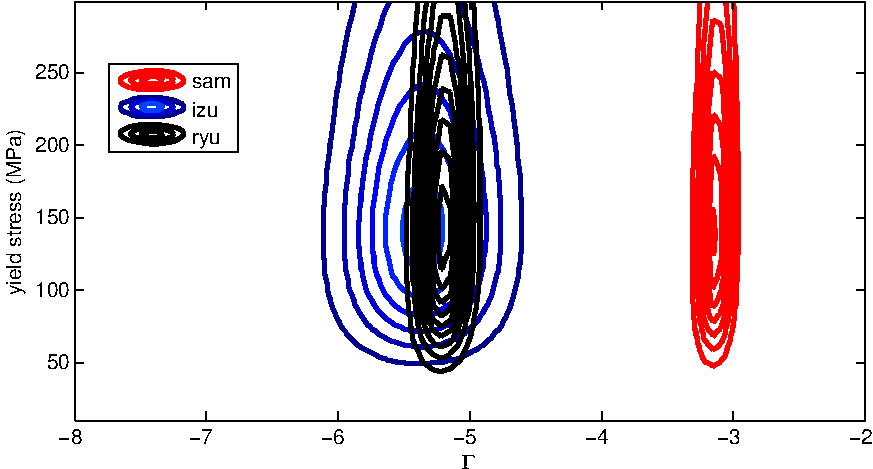
\includegraphics[height=35mm,width=52mm]{gauss_weak_yield.pdf}%{mesh.pdf}
}
\hspace{-0.1cm}\subfigure[]{
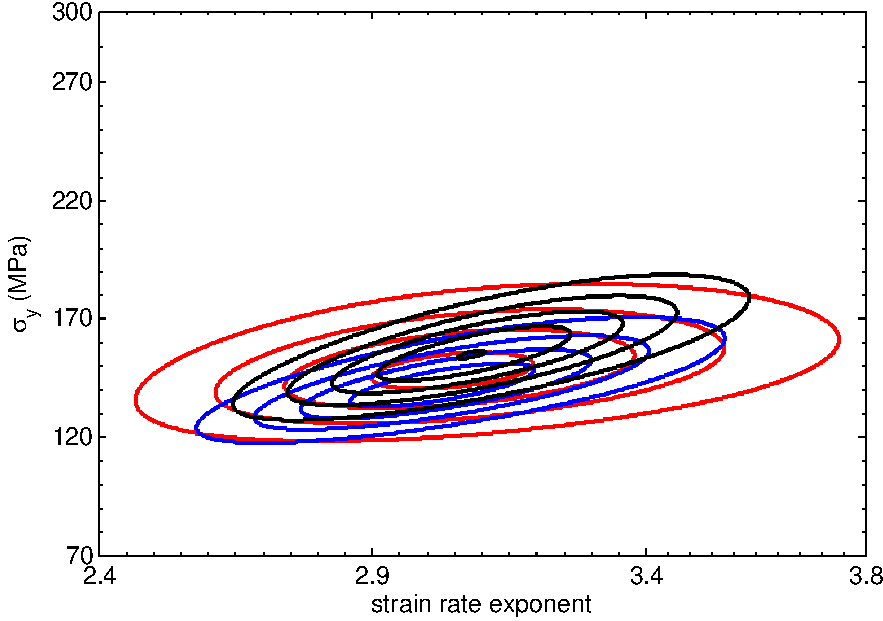
\includegraphics[height=35mm,width=52mm]{paper_cond4.pdf}%{mesh.pdf}
}
\subfigure[]{
\hspace{-0.8cm}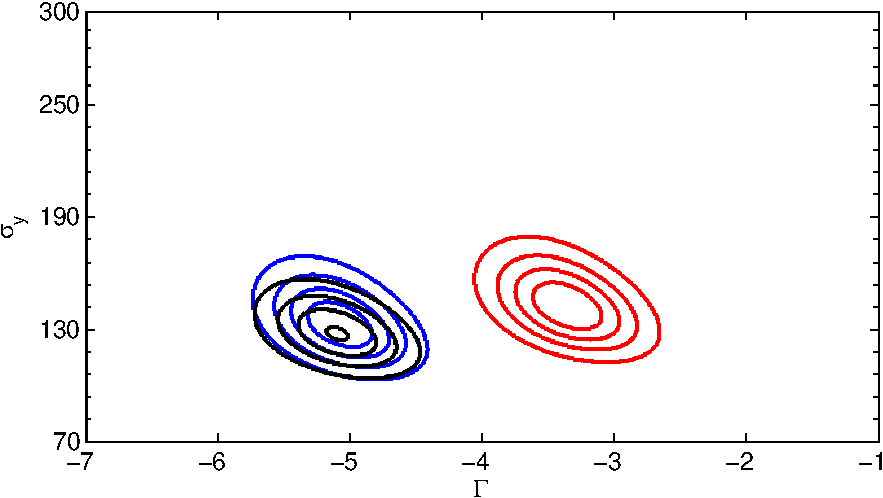
\includegraphics[height=35mm,width=52mm]{paper_cond1.pdf}%{mesh.pdf}
}
\subfigure[]{
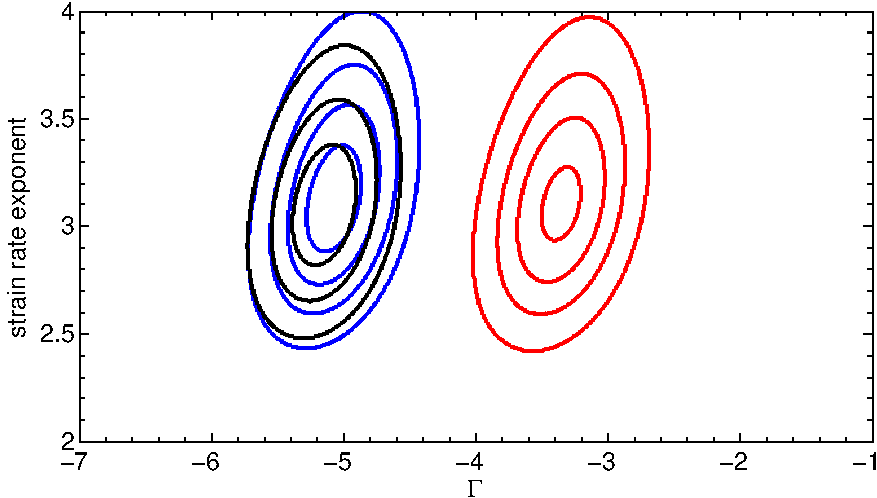
\includegraphics[height=35mm,width=52mm]{paper_cond2.pdf}%{mesh.pdf}
}
\hspace{0.1cm}\subfigure[]{
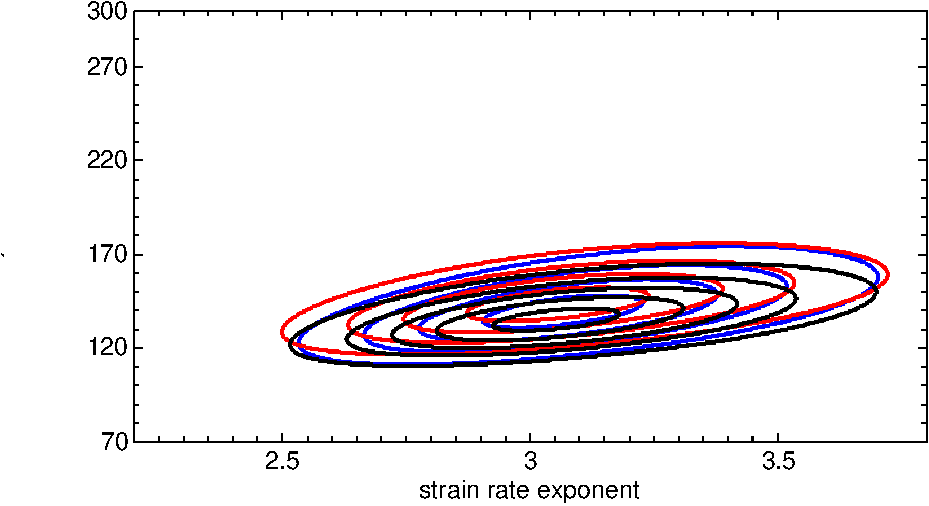
\includegraphics[height=35mm,width=52mm]{paper_cond3.pdf}%{mesh.pdf}
}
%\hspace{-0.2cm}\subfigure[]{
%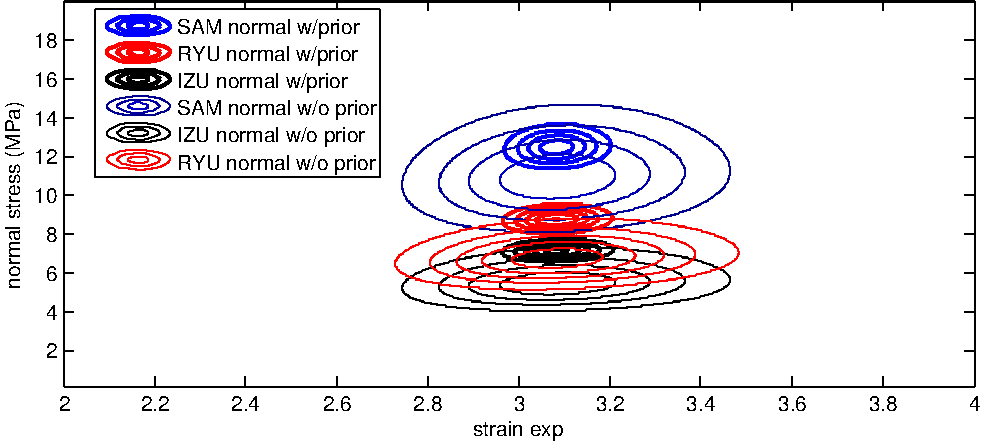
\includegraphics[height=35mm,width=58mm]{normal_comparison_prior2.pdf}%{mesh.pdf}
%}
%\hspace{-0.2cm}\subfigure[]{
%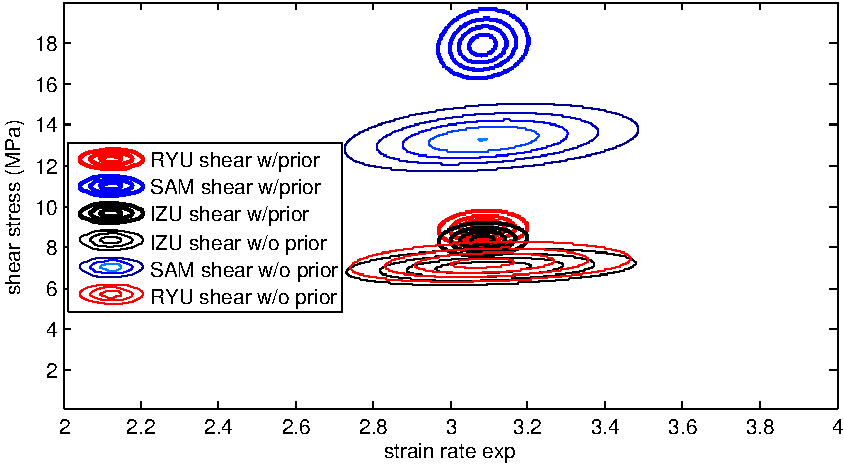
\includegraphics[height=35mm,width=58mm]{shear_comparison_prior.pdf}%{mesh.pdf}
%}
\caption{(a)Strain rate exponent vs plate coupling (b) Yield stress vs plate coupling (c) Yield stress vs. strain rate exponent for Case 1 (South America, Ryukyu and Izu-Bonin-(red:velocity, black:velocity+viscosity, blue:velocity+priors) (d)Strain rate exponent vs plate coupling (e) Yield stress vs plate coupling (f) Yield stress vs. strain rate exponent  (Sumatra (red), Tonga (black) and Central America(blue))}
\label{fig:distrib}
\end{figure}

%An important idea is to know if these trade-offs exist for all inversions, that is with more (or less) inferred parameters, would these correlations remain the same. We find that these trade-offs are consistent when we reduce the parameter space in Case 2, i.e. marginalizing out the upper mantle prefactor, that this there still exists a negative correlation between yield stress and plate coupling in Case 2, which suggests that these rheological parameters are correlated in this way due to the underlying physics with respect to plate motions. Furthermore, we find that there is a positive correlation between the strain rate exponent and yield stress, implying that an increase in strain rate exponent (weakening of the upper mantle) precipitates an increase in yield stress (reduction in plate motion) to make plates resistant to bending.    

An open question about parameter trade-offs deals with additional data, more specifically the average effective viscosity in certain regions of the mantle. 
It is not apparent if these trade-offs will exist with additional data due to the different effects each parameter on both plate motions and average effective viscosity, even though we find similar values for the \textbf{MAP} point between the Case  (without effective viscosity data) and Case 3 (with effective viscosity data). In Fig.\ref{fig:distrib}c we see that the overall distributions are similar in that the trade-offs are the same; however, with the reduction in the variance for the strain rate exponent, the conditional distribution for the strain rate exponent and yield stress, when using average effective viscosity data, is smaller. This result supports the idea that the additional piece of effective viscosity data acts as prior information that can reduce the uncertainty of the inferred parameters. 

While the correlations between the rheological parameters is important, using prior knowledge can further reduce the variance for the inferred rheological parameters. Using prior knowledge from laboratory experiments \citep{korenaga2008new}, we are able to reduce the variance of the plate couplings and global parameters in Case 4 as shown in Fig.\ref{fig:distrib}c, while retaining the same trade-offs between each rheological parameters, which is expected as we only reduced the acceptable range of the inferred parameters. While the conditional distributions for the larger cross-section show that there is indeed trade-offs in plate couplings and global parameters, is is unknown if these trade-offs exist for all subduction zones. To this end, we compared the conditional distributions for Sumatra, Tonga and Central America in Fig.\ref{fig:distrib}d,e and f. 
%\begin{figure}[H]
%\centering
%\hspace{-0.2cm}\subfigure[Weak factor vs. strain rate exponent]{
%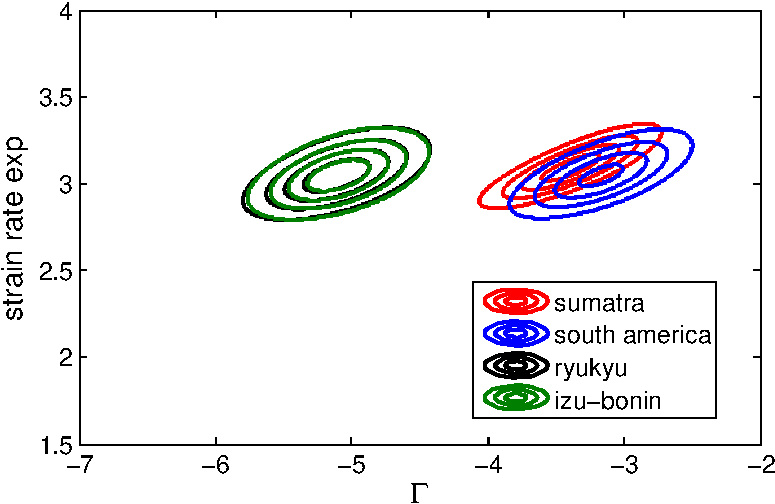
\includegraphics[height=35mm,width=58mm]{gamma_sexp_comp.pdf}%{mesh.pdf}
%}
%\hspace{-0.2cm}\subfigure[Weak Factor vs. yield stress]{
%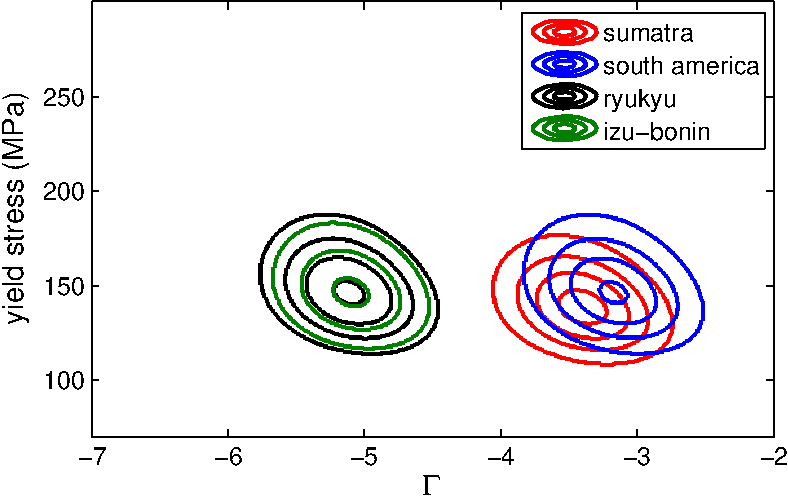
\includegraphics[height=35mm,width=58mm]{gamma_yield_comp.pdf}%{mesh.pdf}
%}
%\hspace{-0.2cm}\subfigure[Weak factor vs. activation energy]{
%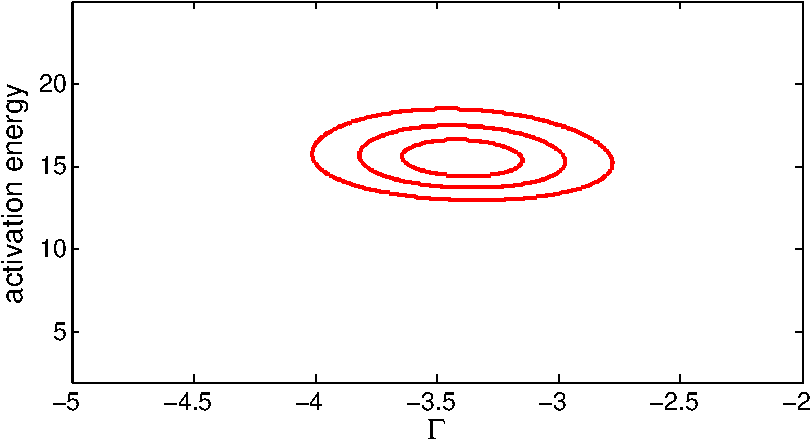
\includegraphics[height=35mm,width=58mm]{gamma_activ_sum.pdf}%{mesh.pdf}
%}
%\hspace{-0.2cm}\subfigure[Yield stress vs. strain rate exponent]{
%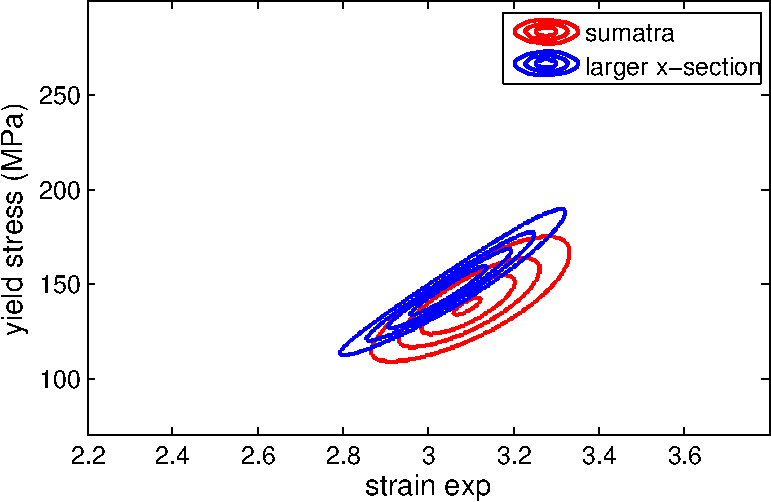
\includegraphics[height=35mm,width=58mm]{yield_strain_comp.pdf}%{mesh.pdf}
%}
%\hspace{-0.2cm}\subfigure[Activation energy vs. strain rate exponent]{
%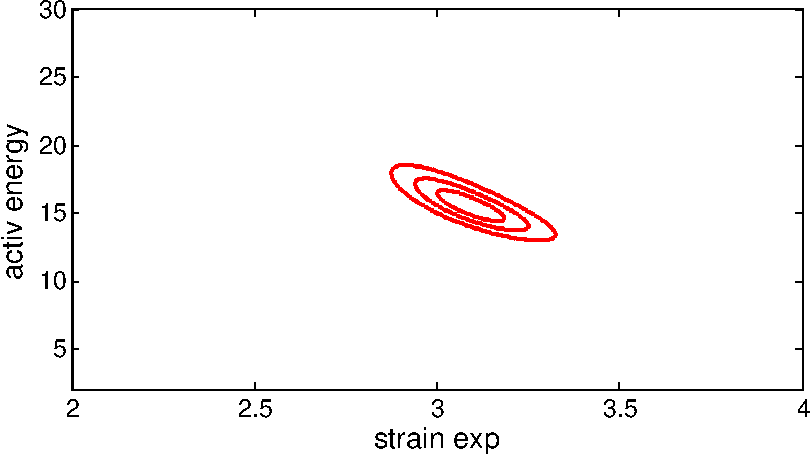
\includegraphics[height=35mm,width=58mm]{activ_strain_sum.pdf}%{mesh.pdf}
%}
%\caption{(a)Weak factor vs. strain rate exponent(b) Weak Factor vs. yield stress (c) Weak factor vs. activation energy %(d)Yield stress vs. strain rate exponent (e)Activation energy vs. strain rate exponent}
%\label{fig:subd_comp}
%\end{figure}

In Fig.\ref{fig:distrib}d-e, we find similar trade-offs between the plate coupling and strain rate exponent, that is an increase in plate coupling (an increase in viscosity within the fault zone) would engender an increase in the strain rate exponent (promotes more shear thinning) so as to increase plate motion. Similarly, as the plate coupling increase the yield stress decreases (promoting more dynamic weakening) so that plates can overcome the resistance from an increase in plate coupling. Furthermore, the same trade-off (positive correlation) between the strain rate exponent and yield stress is found for the Sumatra, Tonga and Central America as shown in Fig.\ref{fig:distrib}f, which seems to suggest that this trade-off between yield stress and strain rate exponent is consistent when it comes to constraining plate motions. Furthermore, there is a similar partitioning of plate coupling in Fig.\ref{fig:distrib}a, b, suggesting that Sumatra will be more coupled compared to Tonga and Central America regardless of the strain rate exponent and yield stress.


One of the key analyses that was developed in this chapter was the characterization of the uncertainty of the stresses (shear and normal) of each plate boundary that is built upon a Gaussian approximation around the \textbf{MAP} point for each inversion. We apply this approach to our models as shown in Fig.\ref{fig:shear_smaller}a,b, where we compare the mean normal and shear stresses of each plate boundary and find that there is a similar pattern of the partitioning between the least coupled subduction zones of Ryukyu and Izu-Bonin to the more coupled subduction zone of South America. Similar to Fig.\ref{fig:distrib}, the same pattern of a more coupled South America plate boundary appears (both normal and shear stresses), regardless of the global parameter. However, we note that the mean of the computed normal stress is lower than the shear stresses, which is certainly not expected.

\begin{figure}[H]
\centering
\hspace{-0.2cm}\subfigure[]{
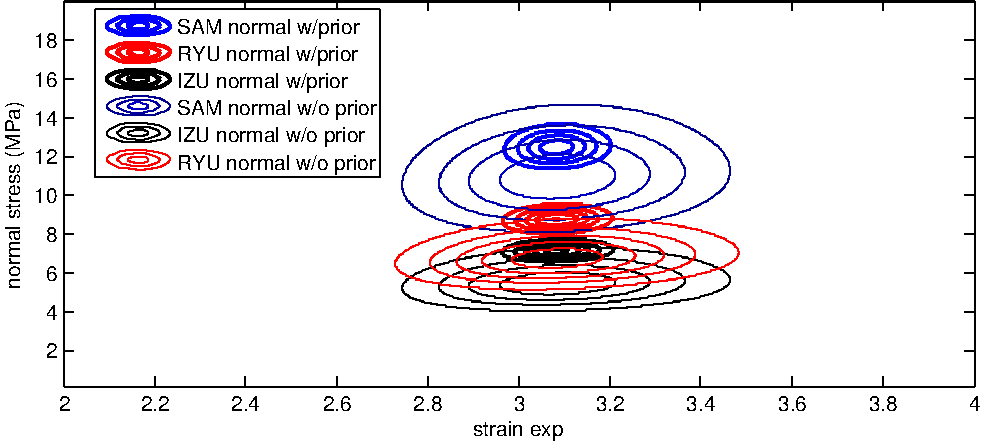
\includegraphics[height=35mm,width=58mm]{normal_comparison_prior2.pdf}%{mesh.pdf}
}
\hspace{-0.2cm}\subfigure[]{
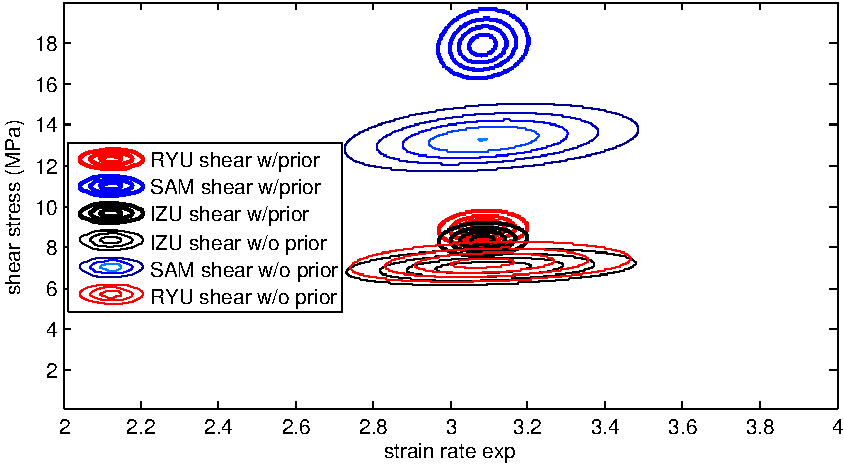
\includegraphics[height=35mm,width=58mm]{shear_comparison_prior.pdf}%{mesh.pdf}
}
\hspace{-0.2cm}\subfigure[normal stresses]{
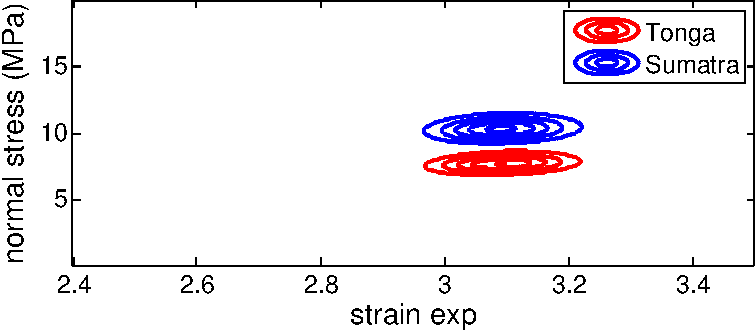
\includegraphics[height=35mm,width=58mm]{normal_tong_sum.pdf}%{mesh.pdf}
}
\hspace{-0.2cm}\subfigure[shear stresses]{
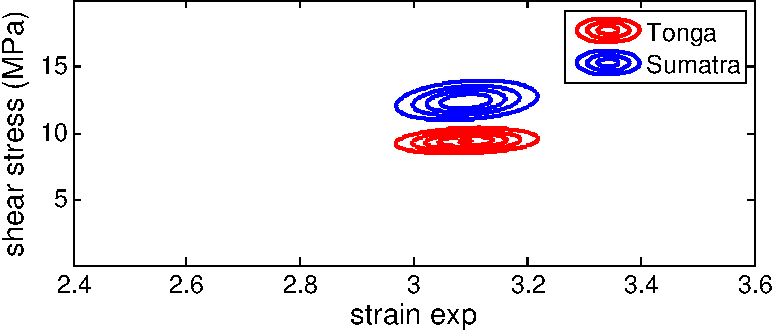
\includegraphics[height=35mm,width=58mm]{shear_tong_sum.pdf}%{mesh.pdf}
}
\caption{(a)Normal stress comparison (d)Shear Stress Comparison for South America, Ryukyu and Izu-Bonin (c)Normal stress comparison (d)Shear Stress Comparison for Tonga and South America}
\label{fig:shear_smaller}
\end{figure}


We similarly compared the stress conditional distributions for Sumatra and Tonga in Fig.\ref{fig:shear_smaller}c,d and find that the shear average shear stress in the fault zones are larger than the normal stress. Similar to South America, we find that there is a partioning of subudction zones for both shear and normal stresses, where Sumatra is more coupled than Tonga.

%\vrnote{Need to do runs with priors without stress-guide}

\section{Discussion}
In our case studies, we explored multiple parameter spaces for subduction zone models that are based on plate motion model data where the rheological parameters are unknown and the observed data is generated from a forward model. Our models from Table \ref{table:inversions} are different from those presented in \citep{ratnaswamy2015adjoint} in that those models are purely synthetic, where the rheolgoical parameters are known. Beginning with Case 1 in Table \ref{table:inversions}, we inferred the global parameters, (including upper mantle prefactor), in addition to plate couplings, and found that there is a clear demarcation in plate boundaries that are more coupled to least coupled. The results from Case 1 has geophysical importance as the inferred plate couplings seems to agree with the variations in seismic coupling from other studies \citep{scholz1995mechanism}.  An important point about our studies in Table \ref{table:inversions}is that we do not know the true values of the inferred parameters, therefore, we rely on how well the data misfit is minimized in addition to how stable the inversions are. Furthermore, we find that the inferred strain rate exponent is slightly larger than 3, while the global yield stress is 148 MPa, which satisfies the bounds from seismicity.

We then test the differences of how the inferred global parameters (strain rate exponent and yield stress) as well as plate couplings change where we no longer infer the upper mantle prefactor, which is akin to what we did in \citep{ratnaswamy2015adjoint} in Case 2. We find that we infer a similar pattern of variations of the couplings of subduction zone, where the Nazca-South America subduction zone is the most coupled. Furthermore, we find that the inferred strain rate exponent is slightly larger than 3.0 just as was found in Case 1, while the global yield stress is of similar value to that of Case 1. Using different pieces of data is important to minimize the uncertainty for the inferred rheological parameters. To this end, we incorporated the average effective viscosity below the South American plate (Case 3).  We find that there is a slightly different value of the yield stress and strain rate exponent than those inferred from Cases 1-2. However, we find that the inferred plate couplings still share the same variation as was found in Cases 1-2 with the Nazca-South America plate boundary being the most coupled, while the Marianas and Ryukyu are less coupled.

Similar to incorporating effective viscosity data, using prior knowledge can help reduce the uncertainty. In Case 4, we make use of our knowledge of the strain rate exponent, yield stress and plate couplings. We found a similar inferred parameters compared to Cases 1-3 for the yield stress and strain rate exponent. Furthermore, the variations in plate couplings remain the same, (South America being the most coupled). We also find that the strain rate exponent is almost the same to our initial guess, while the inferred yield stress is larger than its initial guess. 

In addition to the the larger cross-section in Cases 1-4, we also inferred parameters for different regions, such as Sumatra in Case 5. For this case, we inferred the global parameters and the plate couplings and found that the global parameters are similar in magnitude to what we inferred in Cases 1-4. It is important to note that even with two different cross-sections, the inferred strain rate exponent are very similar. In Case 6, we now add the activation energy as an unknown parameter and find that the strain rate exponent did not increase as much from Case 5. Furthermore, the yield stress still remains within the bounds from seismicity which was similarly observed in Cases 1-5. Another cross-section that we investigated was Tonga, one of the least seismically coupled subduction zones. We similarly (Case 7), inferred the plate coupling and global rheological parameters and found similar values for the inferred yield stress and strain rate exponent compared to Cases 1-6. Furthermore, the plate coupling for Tonga is smaller compared to Sumatra and South America. 

While inferring the rheological parameters is an important outcome of these case studies, the analysis of the uncertainty of the inferred parameters is just as important. 
For Case 1, we look at the conditional distributions such as the strain rate exponent and yield stress vs. the upper mantle prefactor. These distributions suggest that there are correlations between these global parameters. As was seen before in \citep{ratnaswamy2015adjoint}, there is a positive correlation between the yield stress and strain rate exponent. This positive correlation between the yield stress and strain rate exponent suggests that as the yield stress is lowered, plates become more deformable, which in turn increases plate velocities. To compensate for this increase, the strain rate exponent would need to decrease, which in turn would increase the viscosity of the upper mantle in order to slow the plates down. 

The upper mantle prefactor is a parameter that we included for our inference in Case 1 and we see that there is a positive correlation between the upper mantle prefactor and the strain rate exponent. The conditional distribution suggests that when the upper mantle prefactor is increased, (resulting in an increase in the effective viscosity), plates move at a smaller velocity. This  effect from the a reduction in plate speed will give rise to an increase in the strain rate exponent, which promotes more shear thinning in the upper mantle, thereby increasing plate motion.


While the conditional distributions are important to gaining a better understanding of the trade-offs between the rheological parameters, the cumulative stresses in the subduction zones can give a stronger understanding of which subduction zones are more coupled. An important avenue we explored was the inferences of the shear and normal stresses. We see that the cumulative normal and shear stress distributions within each plate boundaries show there is a larger normal and shear stress for South America compared to the Marianas and Ryukyu subduction zones. Furthermore, we note that these plate couplings seem to be independent of the global rheological parameters such as the strain rate exponent and yield stress.  We also find that for the smaller subduction zones, (Sumatra and Tonga), the inferred yield stress and strain rate exponent is approximately the same compared to those that were inferred for the larger cross-section. It should be noted, that these models are 2D approximations to a global flow model, and therefore should not be held as a justification that the inferred rheological parameters and plate couplings from a global flow model will be the same.

Ultimately, we have shown that using the adjoint formulation to efficiently compute gradients for a realistic nonlinear mantle flow model can provide estimates of the rheological parameters and their uncertainties. Furthermore, we are able to incorporate average effective viscosity data for available regions by extending our adjoint formulation. Using the adjoint and an approximation of the Hessian for the covariance matrix, we are able to extend our understanding of the multiple trade-offs of the inferred rheolgical parameters for the 2D cross-sectional models presented. These methods are readily applicable to global models that can capture the complexity of the flow patterns in the mantle, which in turn can aid in the understanding of the relationship between great earthquakes and where they occur from a plate tectonics point of view.


%\section*{Conclusion}

\bibliography{references}


\end{document}

